%-------------------------------------------------------------------------------
% Preamble
%-------------------------------------------------------------------------------

\documentclass[a4paper, 12pt]{article}
\usepackage[margin=2cm]{geometry}
\usepackage[osf]{mathpazo} % palatino
%\usepackage[round]{natbib} % author-year citations
\usepackage[superscript,biblabel,nomove]{cite} % for superscript citations
\usepackage{graphicx}
\usepackage{subcaption}
\usepackage{parskip} 
\usepackage{amsmath}
\usepackage{longtable}
\usepackage{pdflscape}
\usepackage{array}
\usepackage{float}
\usepackage{url}
\usepackage{array}

\pagenumbering{arabic}  
\linespread{1.3}

% figure numbering override
\renewcommand*{\thefigure}{A\arabic{figure}} % make Fig A1 not Fig 1
\renewcommand*{\thetable}{A\arabic{table}} % make Table A1 not Table 1

%-------------------------------------------------------------------------------
% Title page information
%-------------------------------------------------------------------------------

\title{Supplementary Materials from: \textit{Microchromosome fusions underpin convergent evolution of chameleon karyotypes}; journal}

\author{Marcello Mezzasalma, Jeffrey W. Streicher, Fabio M. Guarino, Marc E.H. Jones,\\ 
Simon P. Loader, Gaetano Odierna and Natalie Cooper}

\date{}

% End of preamble

\begin{document}

\maketitle

\tableofcontents

\parindent = 1.5em
\addtolength{\parskip}{.3em}

%-------------------------------------------------------------------------------
% Supplementary materials
%-------------------------------------------------------------------------------

%-----------------------------------------------------------------------------------
% figures 
%-----------------------------------------------------------------------------------
\newpage
\section{Supplementary Figures}

% figure s1
\begin{figure}[H]
 \centering
  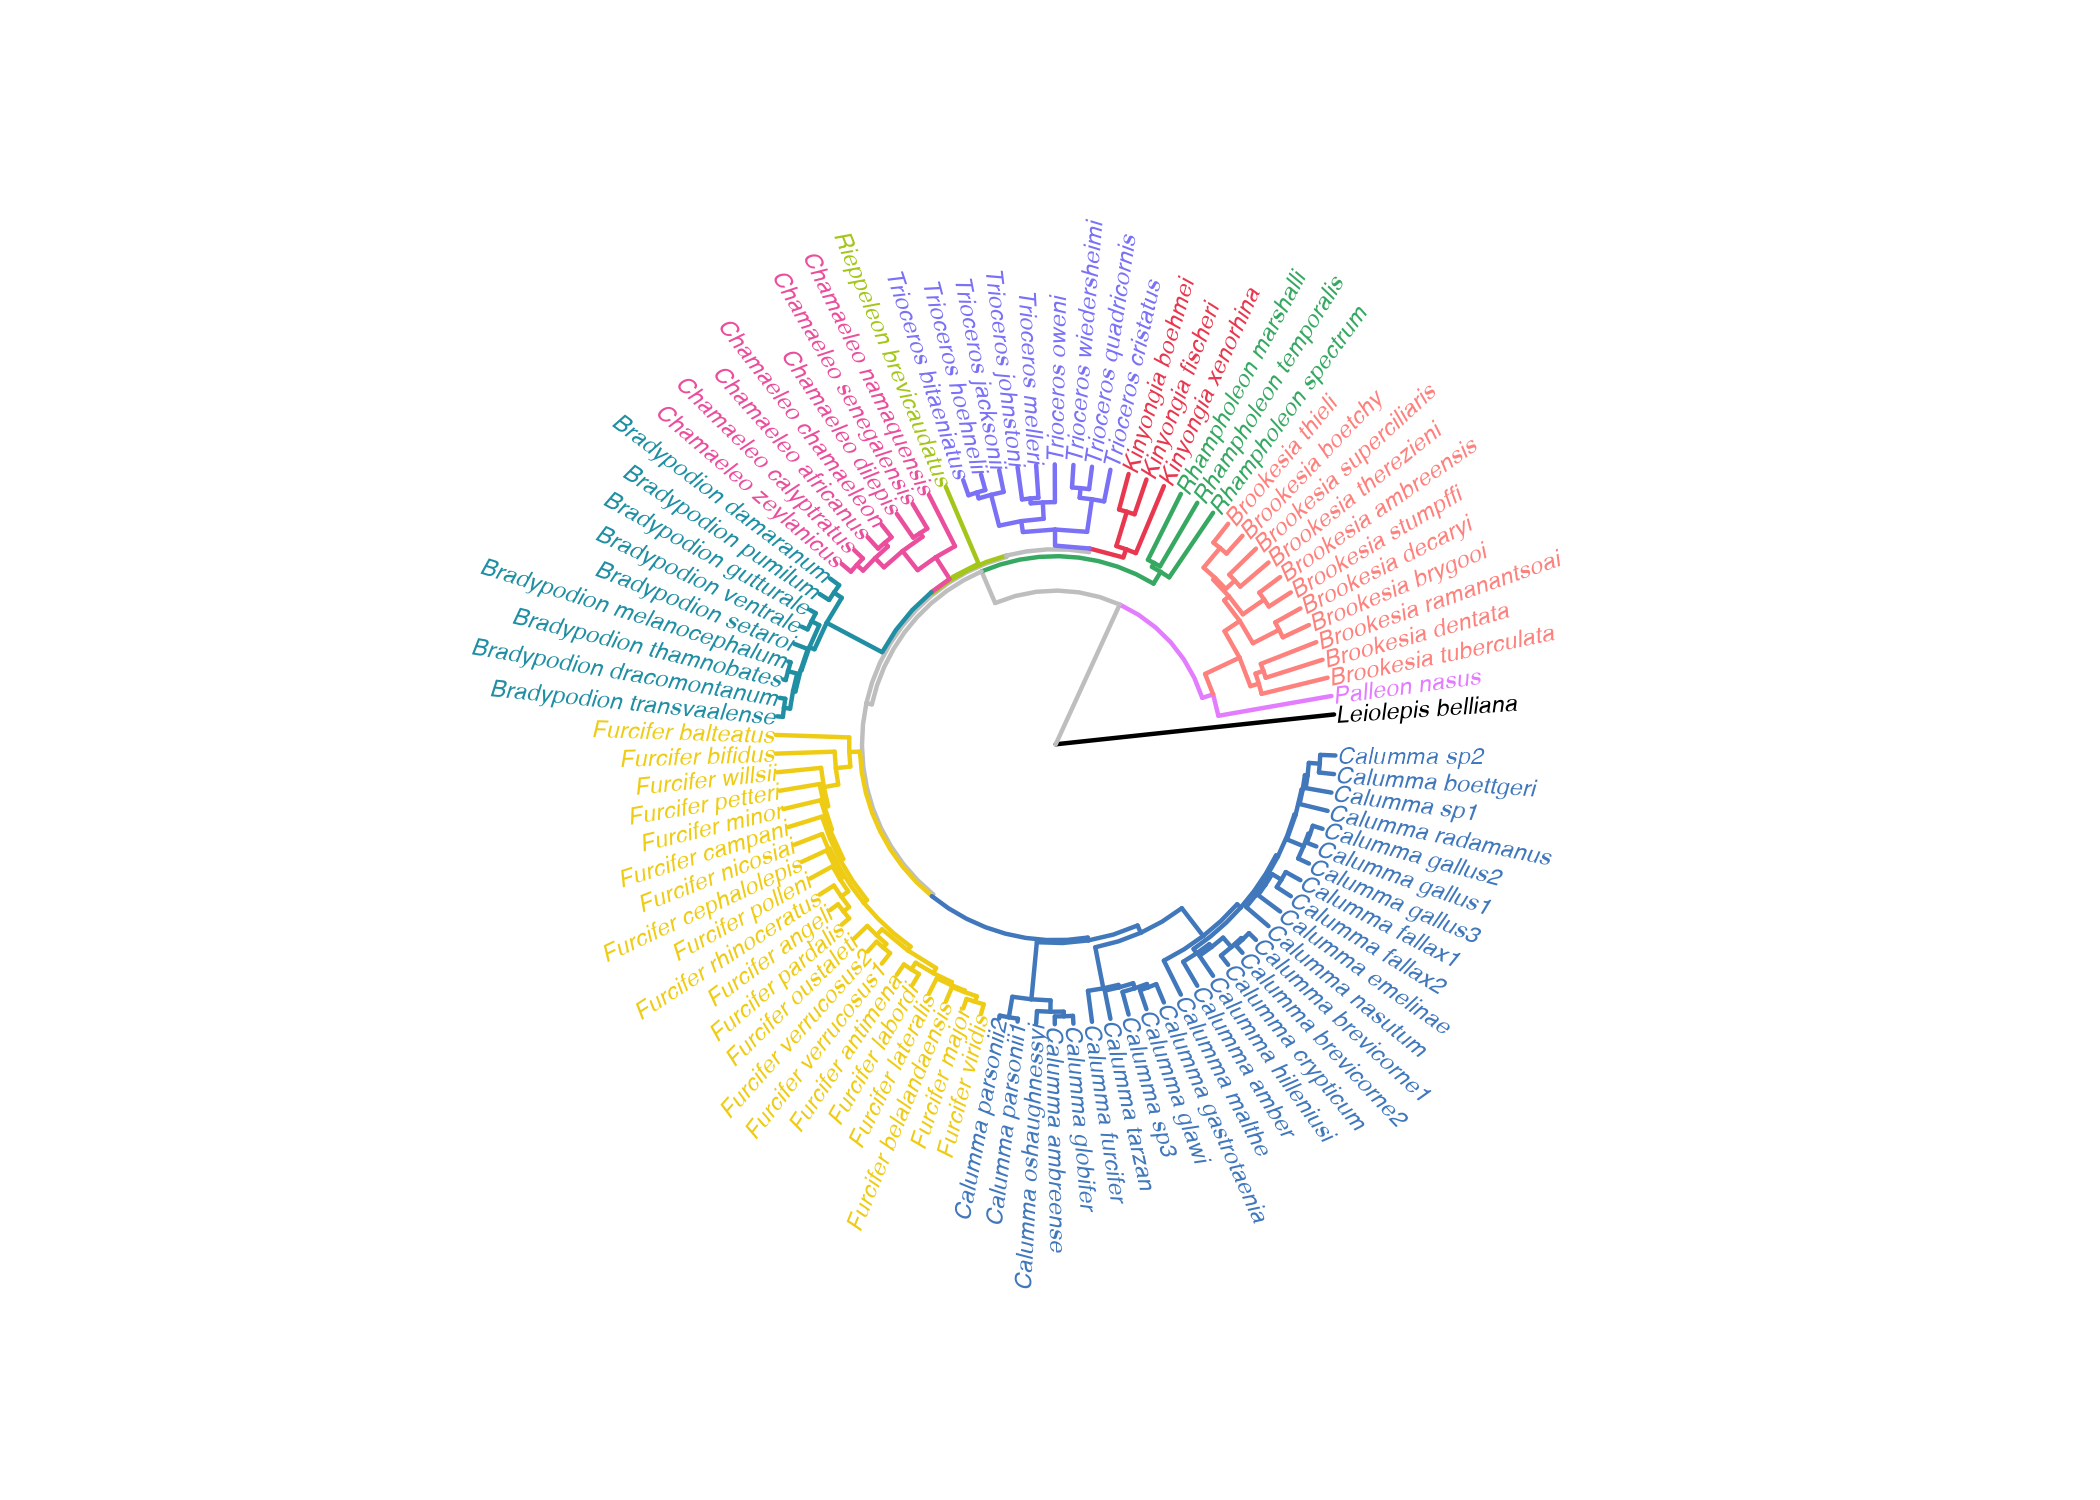
\includegraphics[width = \linewidth]{figures/trees-genera-colour.png}
  \caption{Time calibrated chameleon phylogeny used in the analyses. 
  Branches for each genus have been coloured back to their most recent common ancestor.
}
  \label{fig-phylo}
\end{figure}

% figure s2
\newpage
\begin{figure}[H]
 \centering
  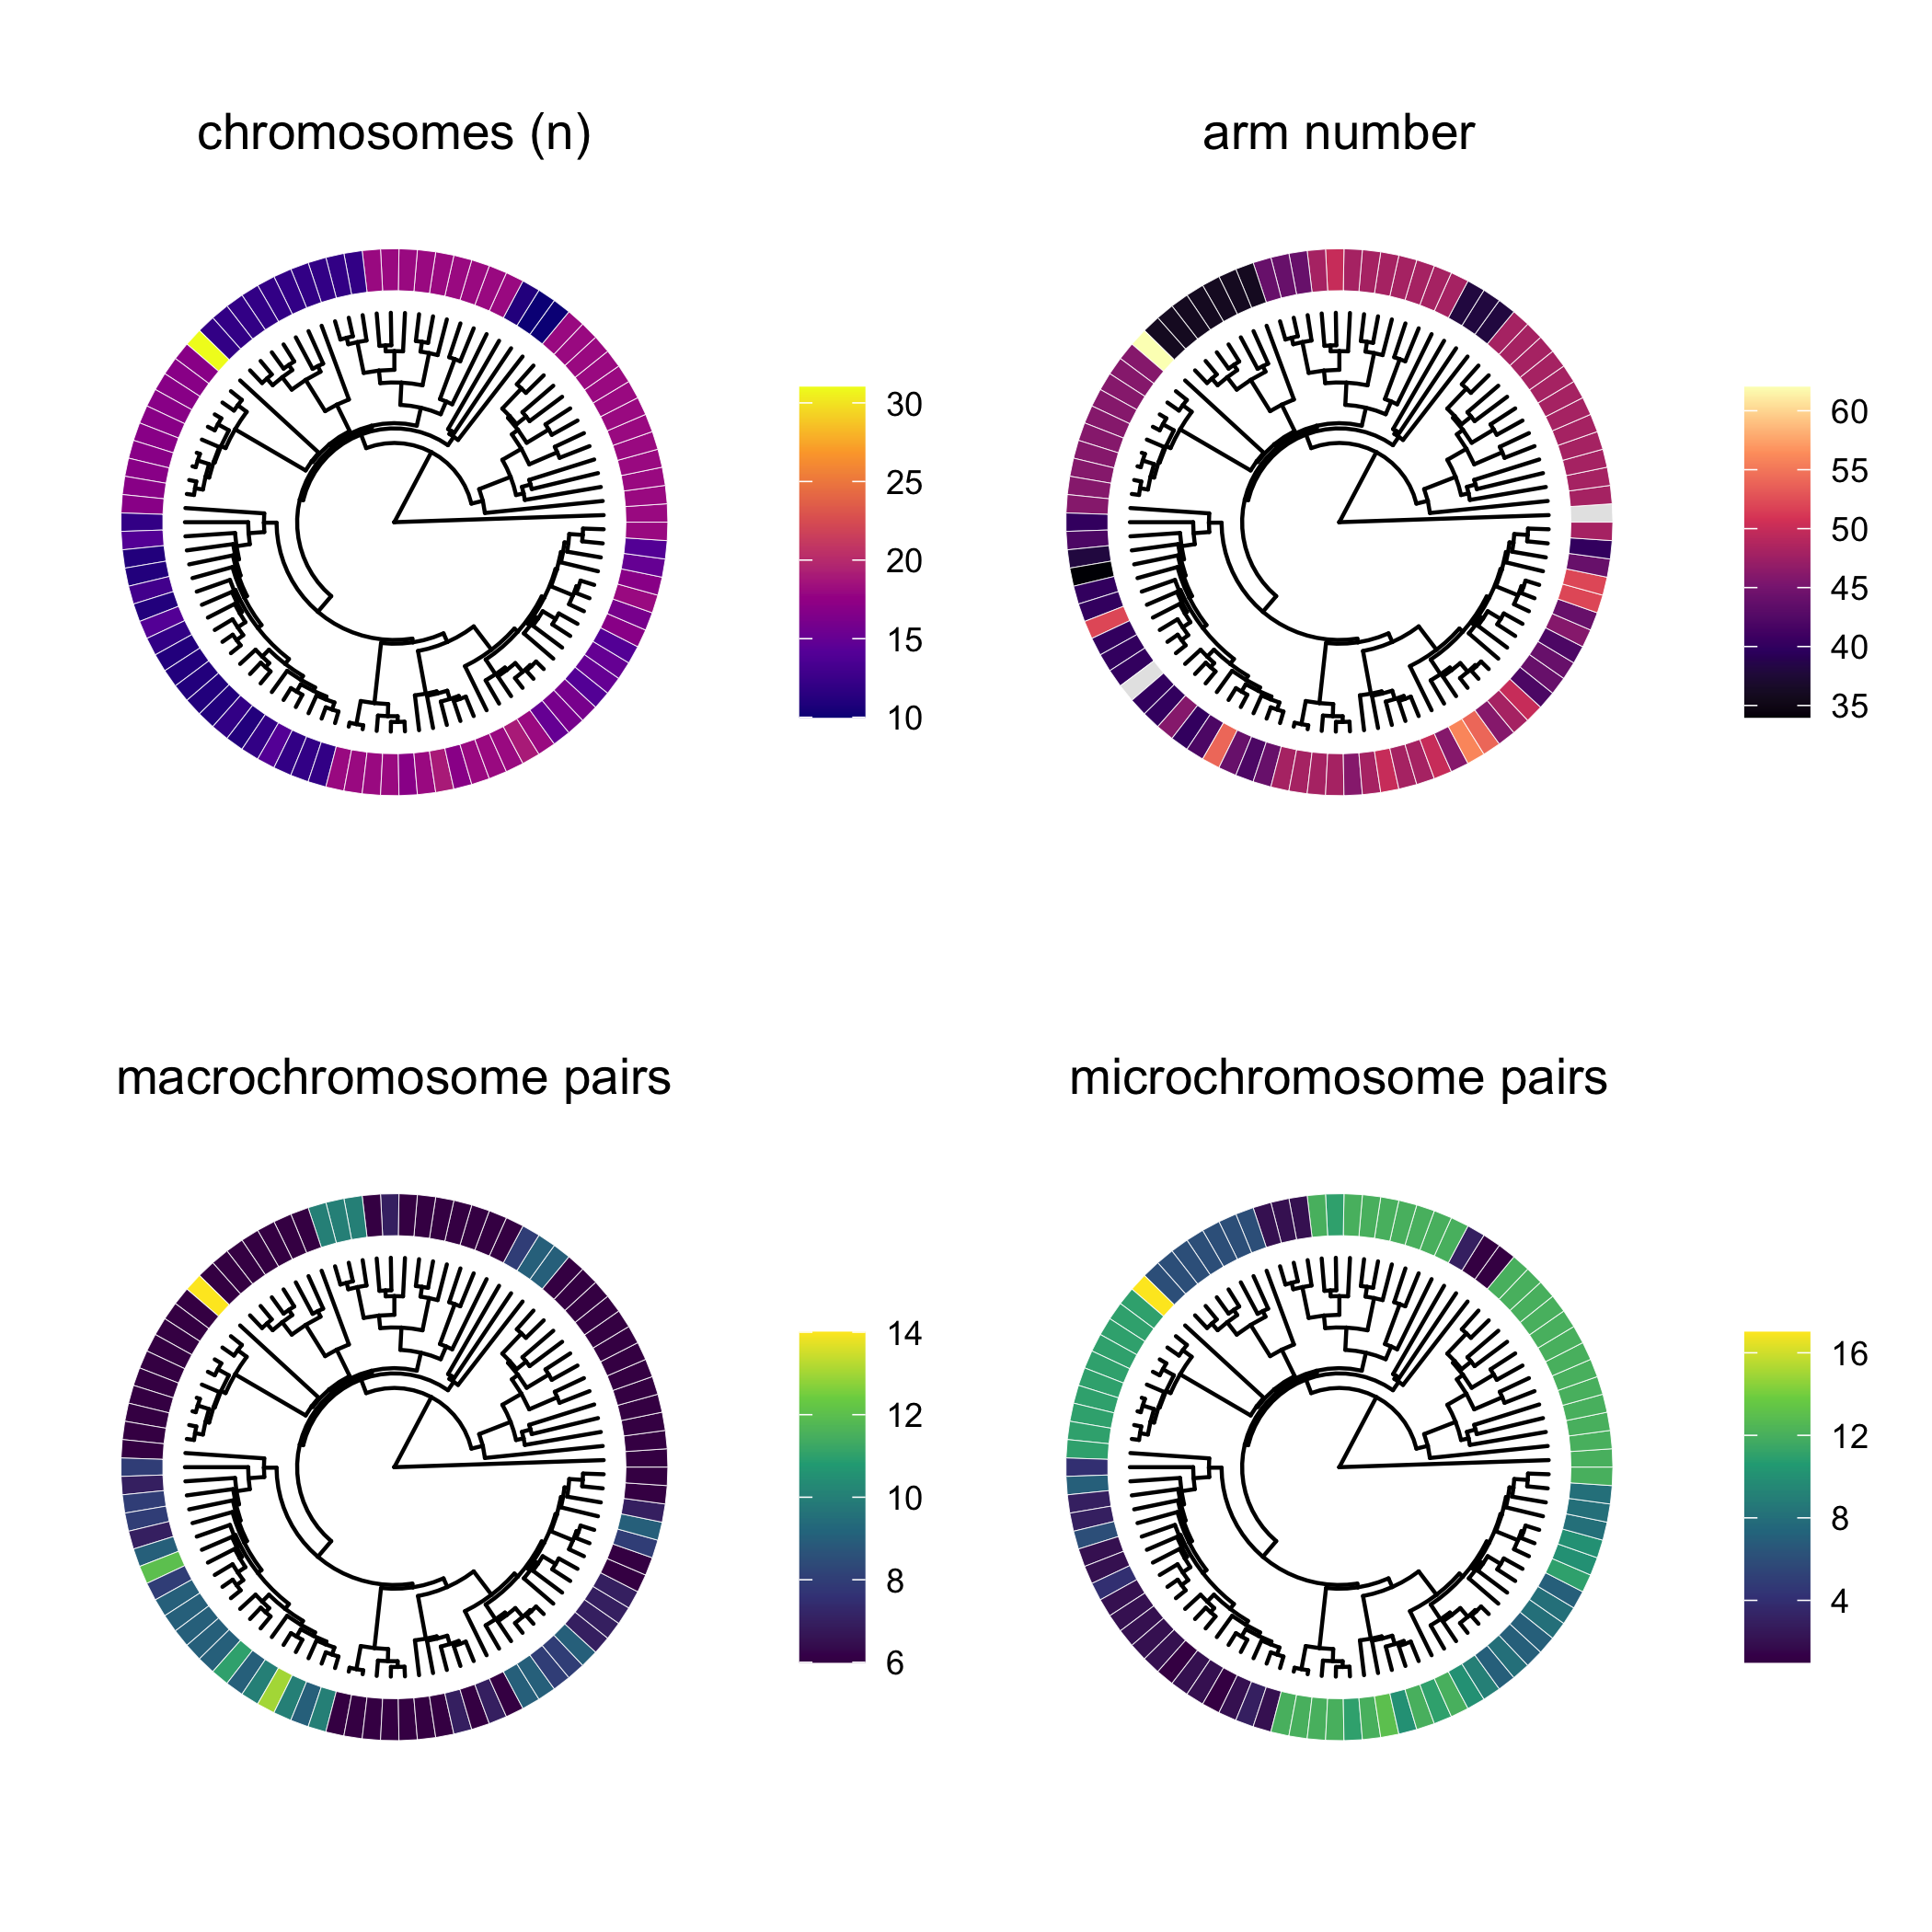
\includegraphics[width = \linewidth]{figures/trees-chromosome-properties.png}
  \caption{Distribution of chromosome properties (haploid number of chromosomes, arm number, number of macrochromosome pairs and number of microchromosome pairs) across the chameleon phylogeny. Note that the scales are different on each plot. The outlier in each case is \textit{Rieppeleon kerstenii} (n = 31). See Figure \ref{fig-phylo} for species identities.
}
  \label{fig-properties}
\end{figure} 

%-----------------------------------------------------------------------------------{}
% duplication analyses
%-----------------------------------------------------------------------------------
\newpage
\section{Chromosome evolutionary models with duplication events}

\subsection{Methods}

We used six additional models to the Constant Rates and Linear Rates models described in the main text that optimise two or more of the following parameters: (i) rate of gain of a single chromosome; (ii) rate of loss of a single chromosome; (iii) polyploidization rate; (iv) demi-polyploidization rate; (v) linear dependency between the current haploid number and the rate of gain chromosomes; and (vi) linear dependency between the current haploid number and the rate of loss chromosomes. Details of which parameters are fitted in each model are shown in Table \ref{table_A1}. All other analysis details are identical to those presented in the text.

% Table A1
\begin{longtable}{lp{0.2\linewidth}p{0.5\linewidth}}

\caption{Details of the eight models fitted in the chromosome evolution analyses.}\\ 
  
\hline
\textbf{Model name} & \textbf{Rate parameters estimated} & \textbf{Interpretation} \\
\hline
CONST\_RATE &
(i) gain, 
(ii) loss,
(iii) polyploidy &
Chromosome numbers change either through gain or loss of single chromosomes, or via whole genome duplication. \\

\hline

CONST\_RATE\_DEMI &
(i) gain, 
(ii) loss, 
(iii) polyploidy = (iv) demipolyploidy &
Chromosome numbers change either through gain or loss of single chromosomes, or via whole genome duplication and half genome duplication. However, the rates of whole genome and half genome duplication are equal.\\

\hline

CONST\_RATE\_DEMI\_EST &
(i) gain,  
(ii) loss, 
(iii) polyploidy,  
(iv) demipolyploidy &
Chromosome numbers change either through gain or loss of single chromosomes, or via whole genome duplication and half genome duplication. \\

\hline

LINEAR\_RATE &
(i) gain,  
(ii) loss, 
(iii) polyploidy, 
(v) gain linear, 
(vi) loss linear &
Chromosome numbers change either through gain or loss of single chromosomes, or via whole genome duplication. Rates for single chromosome gain or loss are dependent on the current chromosome number. \\

\hline

LINEAR\_RATE\_DEMI &
(i) gain,  
(ii) loss, 
(iii) polyploidy = (iv) demipolyploidy,  
(v) gain linear, 
(vi) loss linear &
Chromosome numbers change either through gain or loss of single chromosomes, or via whole genome duplication and half genome duplication. However, the rates of whole genome and half genome duplication are equal. Rates for single chromosome gain or loss are dependent on the current chromosome number. \\

\hline

LINEAR\_RATE\_DEMI\_EST &
(i) gain,  
(ii) loss, 
(iii) polyploidy, 
(iv) demipolyploidy, 
(v) gain linear, 
(vi) loss linear &
Chromosome numbers change either through gain or loss of single chromosomes, or via whole genome duplication and half genome duplication. Rates for single chromosome gain or loss are dependent on the current chromosome number. \\

\hline

\label{table_A1}
\end{longtable}


\subsection{Results}

For models where duplications and demi-duplications were allowed, if \textit{Rieppeleon kerstenii} was included, the Constant Rates with duplications (and demi-duplications for estimated root frequencies) fitted best (Table \ref{table-dup-results}). If \textit{Rieppeleon kerstenii} was excluded, the best fitting model was a Constant Rates model for the fixed root frequencies, and a Constant Rates model with duplications and demi-duplications when we estimated the root frequencies (Table \ref{table-dup-results}). Overall, the best fitting model was the Constant Rates model with duplications and demi-duplications where \textit{Rieppeleon kerstenii} was excluded, and the root was estimated (AIC = 307.1; Table \ref{table-dup-results}; Figure \ref{fig-dup}).

% Table A2
\begin{longtable}{lllll}

\caption{Results from the full set of chromosome evolution models. AIC = Akaike Information Criterion. AICw = AIC weights. AIC and AICw values for the best fitting model in each model set are in bold.}\\ 
  
\hline
\textbf{root} & \textbf{\textit{Rieppeleon?}} & \textbf{model} & \textbf{AIC} & \textbf{AICw} \\
\hline
Iguania &
Yes &
CONST\_RATE  &
\textbf{337.6} &
\textbf{0.518} \\
Iguania &
Yes &
CONST\_RATE\_DEMI &
338.9 &
0.271\\
Iguania &
Yes &
CONST\_RATE\_DEMI\_EST &
339.8 &
0.173\\
Iguania &
Yes &
CONST\_RATE\_NO\_DUPL &
362.0 &
0\\
Iguania &
Yes &
LINEAR\_RATE &
344.1 &
0.020\\
Iguania &
Yes &
LINEAR\_RATE\_DEMI &
345.3 &
0.011\\
Iguania &
Yes &
LINEAR\_RATE\_DEMI\_EST &
346.1 &
0.007 \\
Iguania &
Yes &
LINEAR\_RATE\_NO\_DUPL &
357.3 &
0\\

\hline

Iguania &
No &
CONST\_RATE &
323.7 &
0.154\\
Iguania &
No &
CONST\_RATE\_DEMI &
323.7 &
0.154\\
Iguania &
No &
CONST\_RATE\_DEMI\_EST &
323.1 &
0.208\\
Iguania &
No &
CONST\_RATE\_NO\_DUPL &
\textbf{321.7} &
\textbf{0.419}\\
Iguania &
No &
LINEAR\_RATE &
329.8 &
0.007 \\
Iguania &
No &
LINEAR\_RATE\_DEMI &
326.9 &
0.031 \\
Iguania &
No &
LINEAR\_RATE\_DEMI\_EST &
329.9 &
0.007 \\
Iguania &
No &
LINEAR\_RATE\_NO\_DUPL &
327.8 &
0.020 \\

\hline

n = 18 &
Yes &
CONST\_RATE &
\textbf{336.9} &
\textbf{0.480}\\
n = 18 &
Yes &
CONST\_RATE\_DEMI &
338.0 &
0.277\\
n = 18 &
Yes &
CONST\_RATE\_DEMI\_EST &
338.7 &
0.195\\
n = 18 &
Yes &
CONST\_RATE\_NO\_DUPL &
362.5 &
0\\
n = 18 &
Yes &
LINEAR\_RATE &
342.5 &
0.029\\
n = 18 &
Yes &
LINEAR\_RATE\_DEMI &
342.5 &
0.029 \\
n = 18 &
Yes &
LINEAR\_RATE\_DEMI\_EST &
343.7 &
0.016\\
n = 18 &
Yes &
LINEAR\_RATE\_NO\_DUPL &
359.0 &
0\\

\hline

n = 18 &
No &
CONST\_RATE &
322.7 &
0.190\\
n = 18 &
No &
CONST\_RATE\_DEMI &
322.7 &
0.190\\
n = 18 &
No &
CONST\_RATE\_DEMI\_EST &
324.7 &
0.070\\
n = 18 &
No &
CONST\_RATE\_NO\_DUPL &
\textbf{320.7} &
\textbf{0.515} \\
n = 18 &
No &
LINEAR\_RATE &
329.3 &
0.007\\
n = 18 &
No &
LINEAR\_RATE\_DEMI &
329.3 &
0.007\\
n = 18 &
No &
LINEAR\_RATE\_DEMI\_EST &
331.0 &
0.003\\
n = 18 &
No &
LINEAR\_RATE\_NO\_DUPL &
327.3 &
0.019\\


\hline

estimated &
Yes &
CONST\_RATE &
337.3 &
0.005\\
estimated &
Yes &
CONST\_RATE\_DEMI &
338.6 &
0.003\\
estimated &
Yes &
CONST\_RATE\_DEMI\_EST &
\textbf{326.8} &
\textbf{0.935}\\
estimated &
Yes &
CONST\_RATE\_NO\_DUPL &
359.1&
0\\
estimated &
Yes &
LINEAR\_RATE &
342.4 &
0\\
estimated &
Yes &
LINEAR\_RATE\_DEMI &
342.1 &
0 \\
estimated &
Yes &
LINEAR\_RATE\_DEMI\_EST &
332.4 &
0.057 \\
estimated &
Yes &
LINEAR\_RATE\_NO\_DUPL &
353.3 &
0 \\

\hline

estimated &
No &
CONST\_RATE &
323.1 &
0.001\\
estimated &
No &
CONST\_RATE\_DEMI &
323.1 &
0.001\\
estimated &
No &
CONST\_RATE\_DEMI\_EST &
\textbf{310.2} &
\textbf{0.944}\\
estimated &
No &
CONST\_RATE\_NO\_DUPL &
321.3 &
0.004\\
estimated &
No &
LINEAR\_RATE &
329.0 &
0\\
estimated &
No &
LINEAR\_RATE\_DEMI &
328.0 &
0\\
estimated &
No &
LINEAR\_RATE\_DEMI\_EST &
316.1 &
0.049\\
estimated &
No &
LINEAR\_RATE\_NO\_DUPL &
326.9 &
0\\

\hline

\label{table-dup-results}
\end{longtable}


% figure s3
\newpage
\begin{figure}[H]
 \centering
  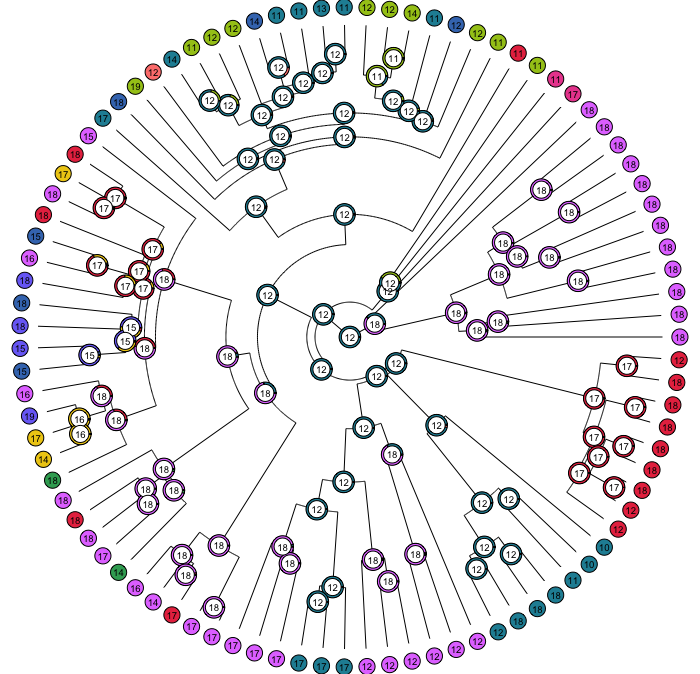
\includegraphics[width = \linewidth]{figures/figure-chromEvol_best-model-all.png}
  \caption{Best fitting model allowing duplications, removing \textit{Rieppeleon kerstenii} and estimating the root node. Numbers at the nodes are the most frequent values obtained from 1,000 simulations. Colours represent the number of chromosomes at the tip, or the proportion of simulations with each number of chromosomes as pie charts at the nodes.
}
  \label{fig-dup}
\end{figure} 

%-----------------------------------------------------------------------------------
% ecology 
%-----------------------------------------------------------------------------------
\newpage
\section{Relationships among chromosome numbers, ecology and life history}

\subsection{Methods}

We tested for correlations between haploid numbers of chromosomes (n) and the following variables; (1) maximum snout vent length (mm; n = 86); (2) substrate (arboreal, terrestrial or multiple; n = 77); (3) reproductive mode (oviparous or viviparous; n = 71); (4) minimum clutch size (eggs; n = 58); (5) maximum clutch size (eggs; n = 58); (6) minimum breeding age (months; n = 43); (7) maximum breeding age (months; n = 43); (8) biogeographic realm (Afrotropical, Madagascar, Oriental or Palearctic; n = 86); (9) absolute latitude (decimal degrees; DD; n = 86). All ecological and life history data were taken from Meiri\cite{meiri2018traits}. Continuous variables were mean-centred and scaled to unit variance prior to analyses.

We used Bayesian phylogenetic generalised mixed models (GLMMs) with Poisson errors in the R package MCMCglmm\cite{hadfield2010mcmc} to test for correlations, including the phylogeny (as the inverse of the phylogenetic variance-covariance matrix) as a random effect to account for phylogenetic autocorrelation. We ran each MCMCglmm model for 1 x 106 iterations sampling at every 1,000 iterations and discarding the first 1 x 105 iterations as burn-in. We used the default priors for MCMCglmm ($μ = 0$ and $V = I × 1010$ for fixed effects and parameter expanded priors, and $V = 1$, $\nu = 1$, $\alpha \mu = 0$, and $\alpha V = 252$ for the phylogenetic random effects). All model parameters had a mean effective sample size (ESS; estimated using the R package coda\cite{plummer2006coda}) of over 800, and traceplots indicated that models had converged.

\subsection{Results}

We found no significant correlations among chromosome numbers and any of our ecology or life history variables (Table \ref{table-ecology}; Figures \ref{fig-ecology1} - \ref{fig-ecology2}). 

% Table A2
\begin{longtable}{llllll}

\caption{Results from Bayesian phylogenetic generalised linear mixed models with Poisson errors, for the relationship between haploid chromosome number in chameleons and several explanatory variables. CI = confidence interval; ESS = effective sample size; n = number of taxa; SVL = snout vent length.}\\ 
  
\hline
\textbf{variable} & \textbf{Posterior mean} & \textbf{Lower 95\% CI} & \textbf{Upper 95\% CI} & \textbf{ESS}& \textbf{n} \\
\hline
max SVL &
-0.031 &
-0.106 &
0.052 &
900 &
86 \\
Substrate terrestrial &
0.010 &
-0.251 &
0.220 &
900 &
83\\
Substrate multiple &
-0.005 &
-0.163 &
0.133 &
999 &
83\\
reproductive mode &
-0.054 &
-0.333 &
0.180 &
800 &
77\\
min clutch size &
0.004 &
-0.069 &
0.084 &
900 &
61\\
max clutch size &
-0.047 &
-0.127 &
0.031 &
900 &
61\\
min breeding age &
0.026 &
-0.064 &
0.110 &
900 &
46\\
max breeding age &
0.007 &
-0.076 &
0.105 &
900 &
46\\
Realm Madagascar &
-0.004 &
-0.176 &
0.182 &
900 &
86\\
latitude &
-0.007 &
-0.089 &
0.061&
900 &
86\\

\hline

\label{table-ecology}
\end{longtable}

% figure
\begin{figure}[H]
 \centering
  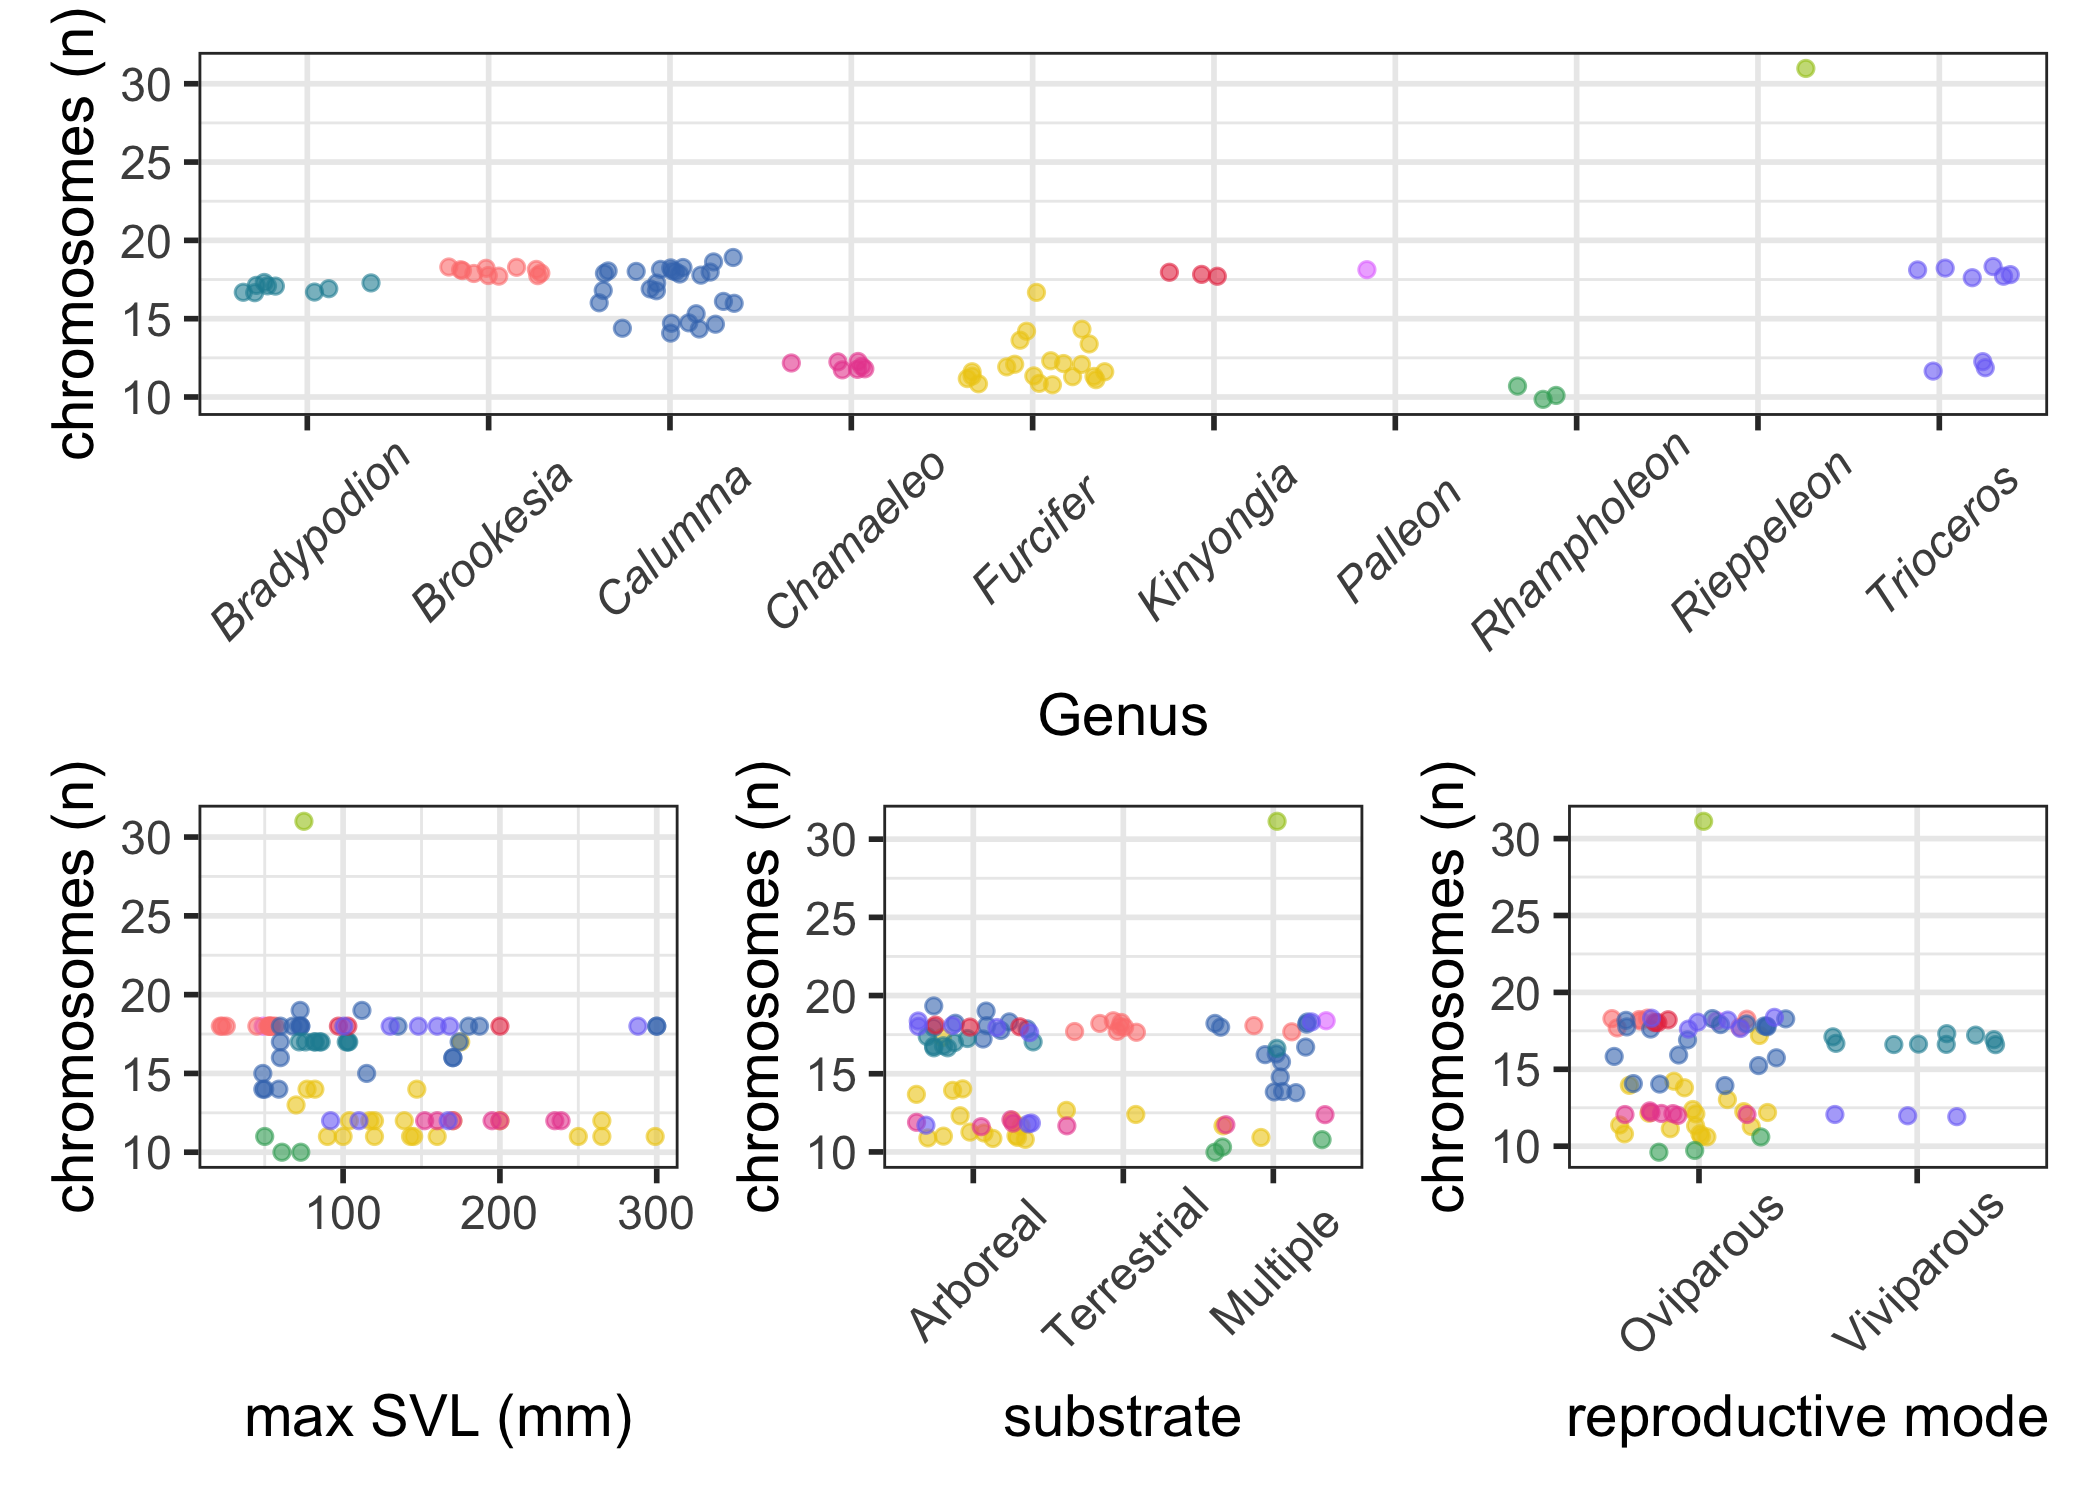
\includegraphics[width = \linewidth]{figures/ecology-genus-svl.png}
  \caption{Relationships between genus (n = 92), maximum snout vent length (SVL; n = 86), substrate (n = 83), reproductive mode (n = 77) and haploid chromosome number in chameleons. Points are coloured by genus as shown in the upper panel. The outlier at n = 31 is \textit{Rieppeleon kerstenii}.
}
  \label{fig-ecology1}
\end{figure} 

\newpage
\begin{figure}[H]
 \centering
  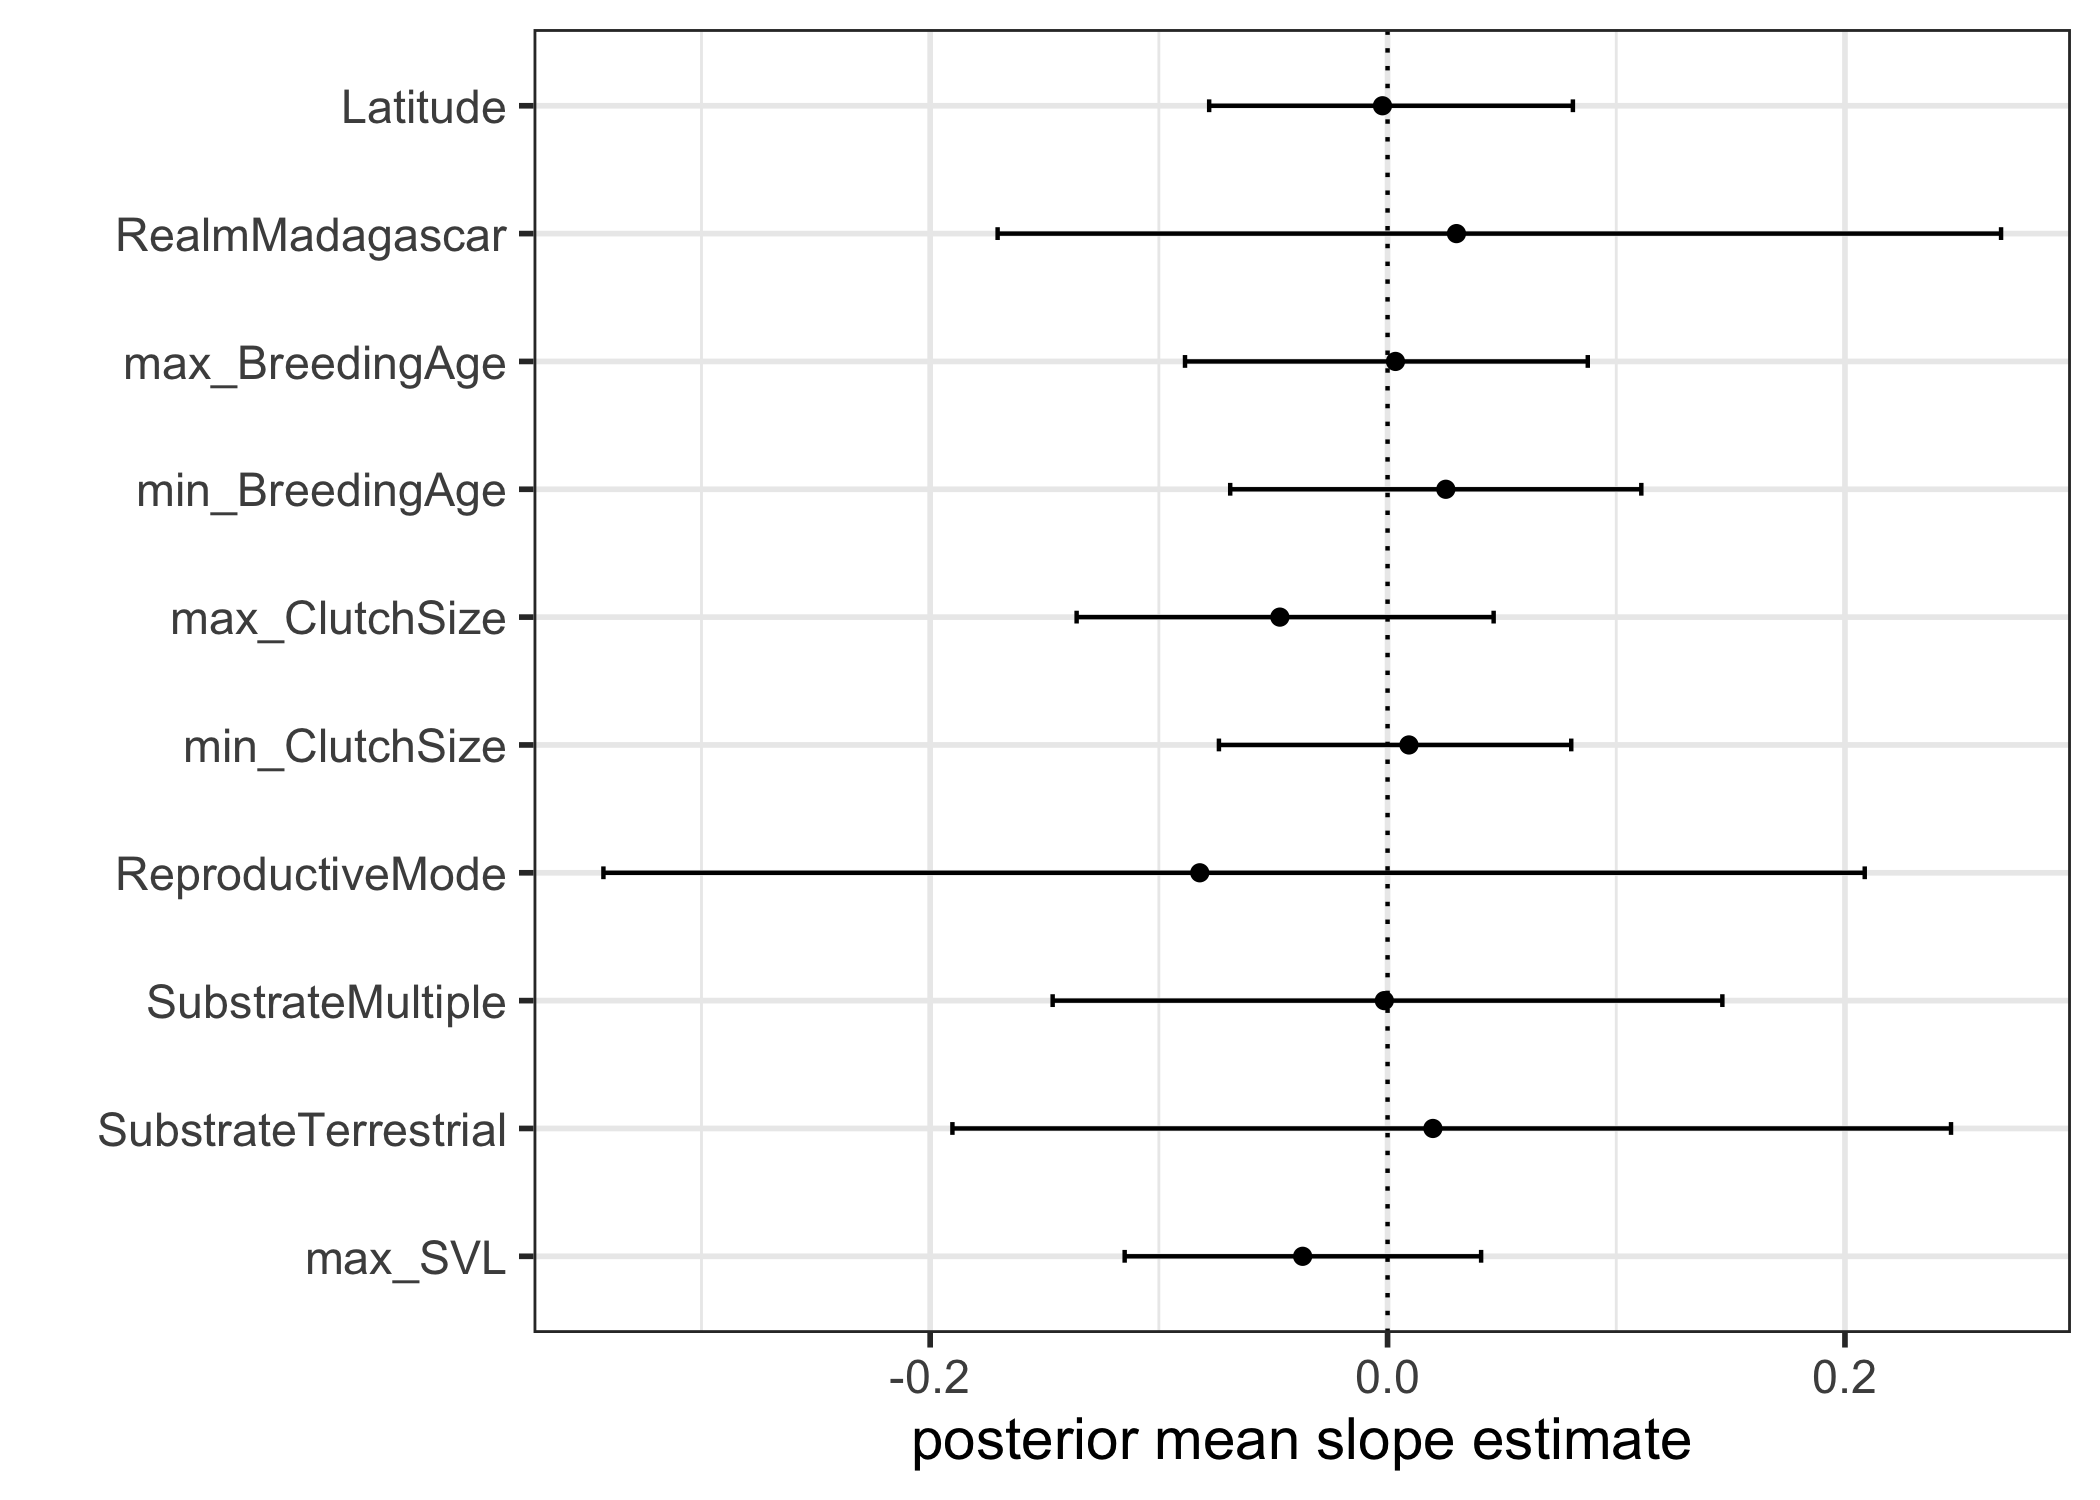
\includegraphics[width = \linewidth]{figures/mcmcglmm-figure.png}
  \caption{Results from Bayesian phylogenetic generalised linear mixed models with Poisson errors, showing posterior means of each slope estimate for the relationship between haploid chromosome number in chameleons and several explanatory variables. max\_SVL.
}
  \label{fig-ecology2}
\end{figure}



%-----------------------------------------------------------------------------------
% otus 
%-----------------------------------------------------------------------------------
\newpage
\section{Results from analyses using all OTUs in the models}

We have molecular and karyotypic data for 137 samples. Most species within the sample have a consistent karyotype, therefore our main analyses use only one representative for each species to avoid pseudoreplication, except for the five taxa which have intraspecific variation in their karyotypes. For completeness we repeated the analyses using all 137 samples.

\subsection{Chromosome evolutionary models}
When \textit{Rieppeleon kerstenii} was included the Linear Rates model fitted better than the Constant Rates model (Table \ref{table-otus}). Although rates of chromosome loss were also consistently higher than rates of chromosome gain in these models, rates of linear dependency between the current haploid number and the rate of loss of chromosomes were lower for loss than gain of chromosomes. This was regardless of root frequencies. The Constant Rates model fitted better than the Linear Rates model when \textit{Rieppeleon kerstenii} was excluded from the analyses, and rates of chromosome loss were consistently higher than rates of chromosome gain in these models (Table \ref{table-otus}). Again, this was regardless of root frequencies. Overall, the best fitting model is the Constant Rates model where \textit{Rieppeleon kerstenii} was excluded, and the root is set to 18 (Figure \ref{fig-otus-models}). 

\noindent For models where duplications and demi-duplications were allowed, if the root is estimated then the best fitting model is a Constant Rates model with both duplications and demi-duplications, regardless of whether \textit{Rieppeleon kerstenii} was excluded or not. For the other root states, the best fitting model is a Constant Rates model with duplications if \textit{Rieppeleon kerstenii} was included, and a Constant Rates model if \textit{Rieppeleon kerstenii} was excluded (Table \ref{table-otus}). 

\newpage
% Table A2
\begin{longtable}{lccccccccc}

\caption{Results from Constant Rates and Linear Rates chromosome evolution models. AIC = Akaike Information Criterion. AIC values for the best fitting model in each model set are in bold. loss = rate of chromosome loss; gain = rate of chromosome gain; lossL = linear dependency between the current haploid number and the rate of loss chromosomes; gainL = linear dependency between the current haploid number and the rate of gain chromosomes.}\\ 
  
\hline
 &  & \multicolumn{3}{c}{\textbf{Constant Rates}} & \multicolumn{5}{c}{\textbf{Linear Rates}} \\
\textbf{root} & \textbf{\textit{Rieppeleon}?} & 
\textbf{AIC} & \textbf{loss} & \textbf{gain} & 
\textbf{AIC} & \textbf{loss} & \textbf{gain} & \textbf{lossL} & \textbf{gainL} \\
\hline
Iguania  &
Yes &
372.5 &
0.081 &
0.087 &
\textbf{367.1} &
0.080 &
0.000 &
0.000 &
0.005 \\
n = 18  &
Yes &
373.0 &
0.090 &
0.080 &
\textbf{367.6} &
0.135 &
0.000 &
-0.003 &
0.004 \\
estimated &
Yes &
371.2 &
0.000 &
0.169 &
\textbf{366.1} &
0.000 &
0.032 &
0.000 &
0.009 \\
Iguania &
No &
\textbf{329.2} &
0.073 &
0.004 &
333.1 &
0.074 &
0.000 &
0.000 &
0.003 \\
n = 18 &
No &
\textbf{328.1} &
0.079 &
0.038 &
329.2 &
0.135 &
0.000 &
-0.003 &
0.004 \\
estimated &
No &
\textbf{328.5} &
0.085 &
0.027 &
331.9 &
0.088 &
0.000 &
-0.001 &
0.002\\
\hline

\label{table-otus}
\end{longtable}

% figure
\begin{figure}[H]
 \centering
  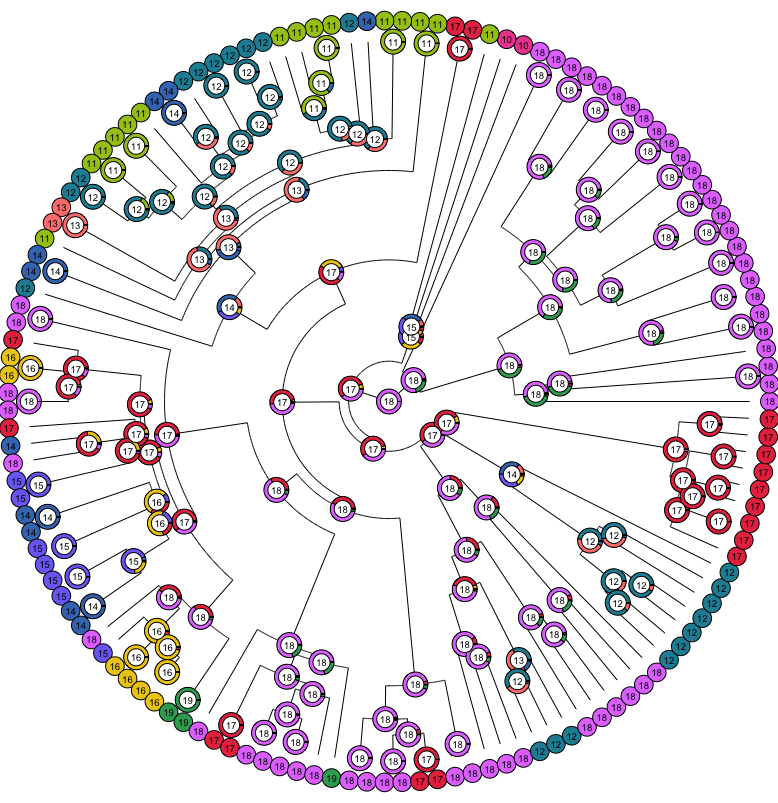
\includegraphics[width = \linewidth]{figures/tree-best-model-taxa.png}
  \caption{Best fitting chromosome evolution model using taxa as tips, removing \textit{Rieppeleon kerstenii} and using n = 18 as the root node. Numbers at the nodes are the most frequent values obtained from 1,000 simulations. Colours represent the number of chromosomes at the tip, or the proportion of simulations with each number of chromosomes as pie charts at the nodes.
}
  \label{fig-otus-models}
\end{figure} 

\subsection{Fissions and fusions and ITS}
There was a significant negative correlation between the haploid number of chromosomes and the number of macrochromosome pairs (GLM: $\chi^2$ = 12.49, df = 1,134, p $<$ 0.001; Figure \ref{fig-otus-macro}A), and a significant positive correlation between the haploid number of chromosomes and the number of microchromosome pairs (GLM: $\chi^2$ = 72.89, df = 1,134, p $<$ 0.001; Figure \ref{fig-otus-macro}B). Additionally, there was a significant relationship between the number of micro- and macro- chromosome pairs (GLM: $\chi^2$ = 169.57, df = 1,134, p $<$ 0.001; Figure \ref{fig-otus-macro}C). There was a significant negative correlation between ITS and the haploid number of chromosomes (GLM: F = 59.91, df = 1,72, p $<$ 0.001; Figure \ref{fig-otus-its}A), a significant positive correlation between ITS and the number of macrochromosome pairs (GLM: F = 16.30, df = 1,72, p $<$ 0.001; Figure \ref{fig-otus-its}B), and a significant relationship between ITS and the number of microchromosome pairs (GLM: F = 61.87, df = 1,72, p $<$ 0.001; Figure \ref{fig-otus-its}C). 

% figure
\begin{figure}[H]
 \centering
  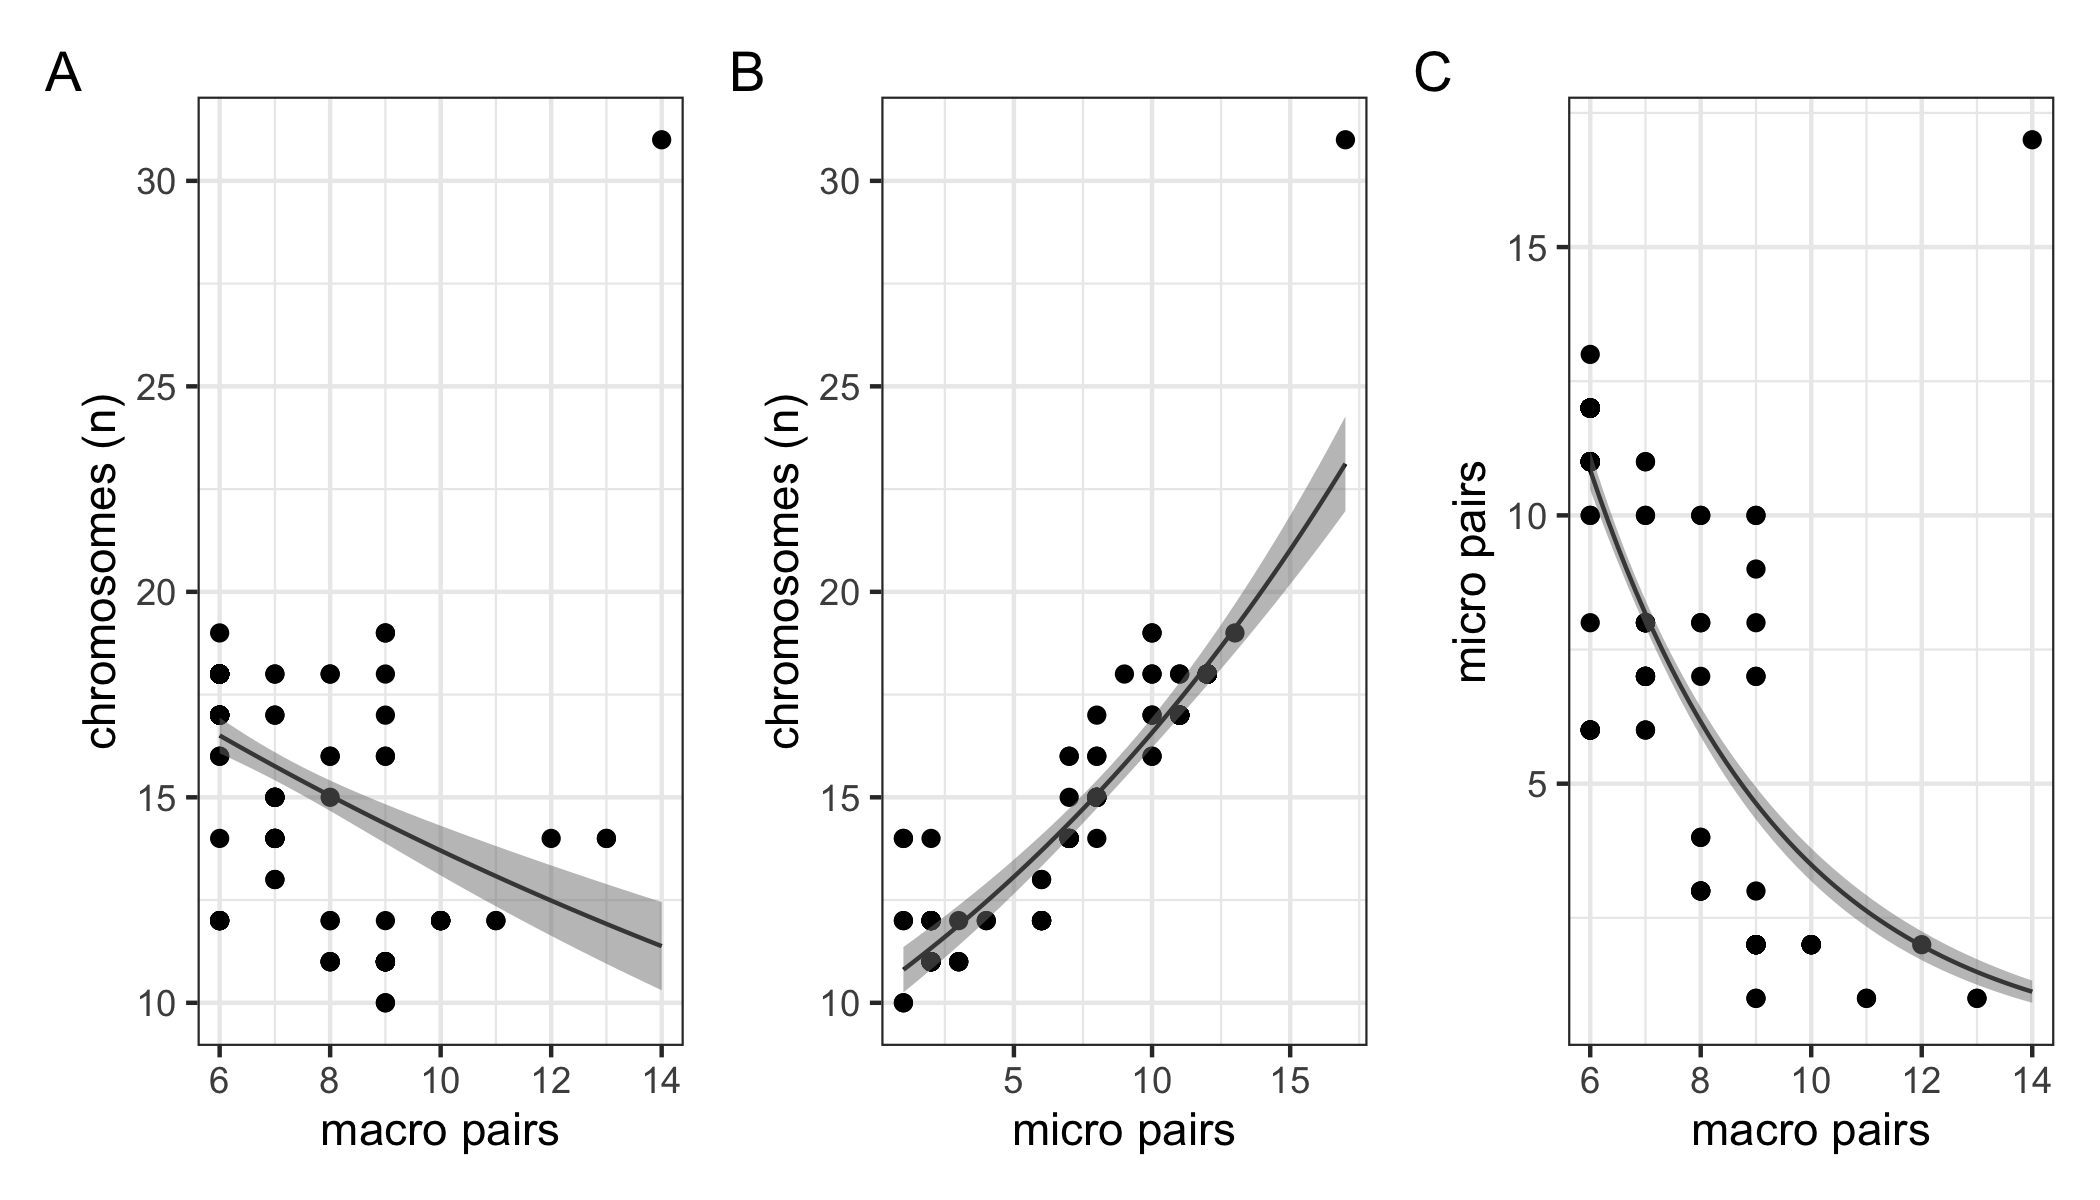
\includegraphics[width = \linewidth]{figures/micro-macro-chromosomes.png}
  \caption{Correlations among the haploid number of chromosomes (n), numbers of macrochromosome pairs and numbers of microchromosome pairs in chameleons. Fitted lines and standard errors are the outputs from generalised linear models with Poisson errors. The outlier at n = 31 is \textit{Rieppeleon kerstenii}.
}
  \label{fig-otus-macro}
\end{figure} 


% figure
\newpage
\begin{figure}[H]
 \centering
  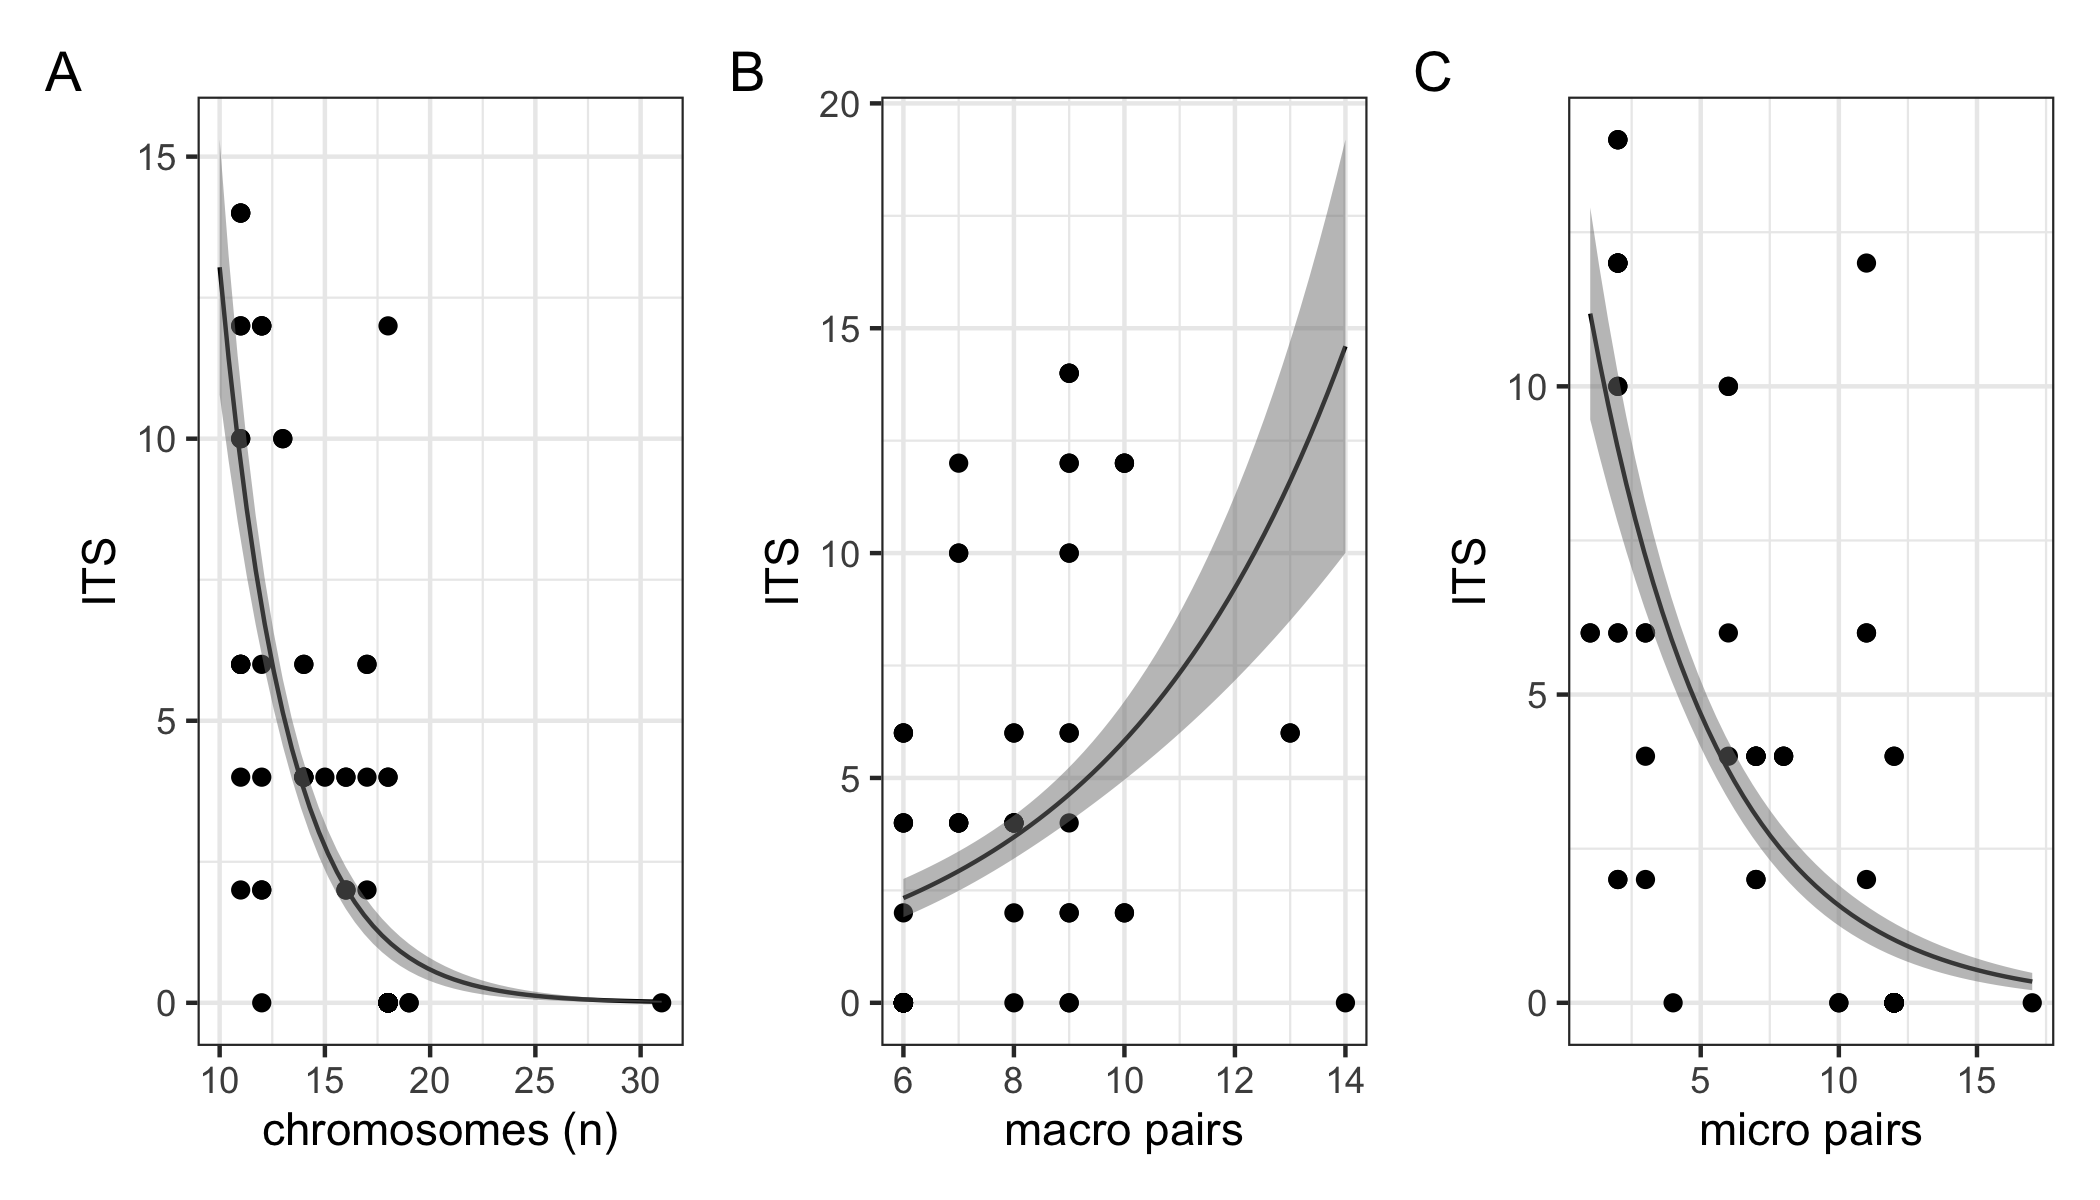
\includegraphics[width = \linewidth]{figures/ITS-chromosomes.png}
  \caption{Correlations among ITS and the haploid number of chromosomes (n), numbers of macrochromosome pairs and numbers of microchromosome pairs in chameleons. Fitted lines and standard errors are the outputs from generalised linear models with quasipoisson errors.
}
  \label{fig-otus-its}
\end{figure} 


\subsection{Phylogenetic patterns}
Differences in chromosome number did not increase with phylogenetic distance (Figure \ref{fig-otus-pairwise}); even some of the most distantly related taxa in our phylogeny shared the same chromosome numbers. Large differences in chromosome numbers, however, only occur at moderate to large phylogenetic distances. Simulations give a reasonable approximation of observed chromosome numbers at the tips of the phylogeny, however, model predictions do not account well for the large numbers of species with n = 11, n = 12 and n = 18 chromosomes (Figure \ref{fig-otus-predicted}). 

% figure
\newpage
\begin{figure}[H]
 \centering
  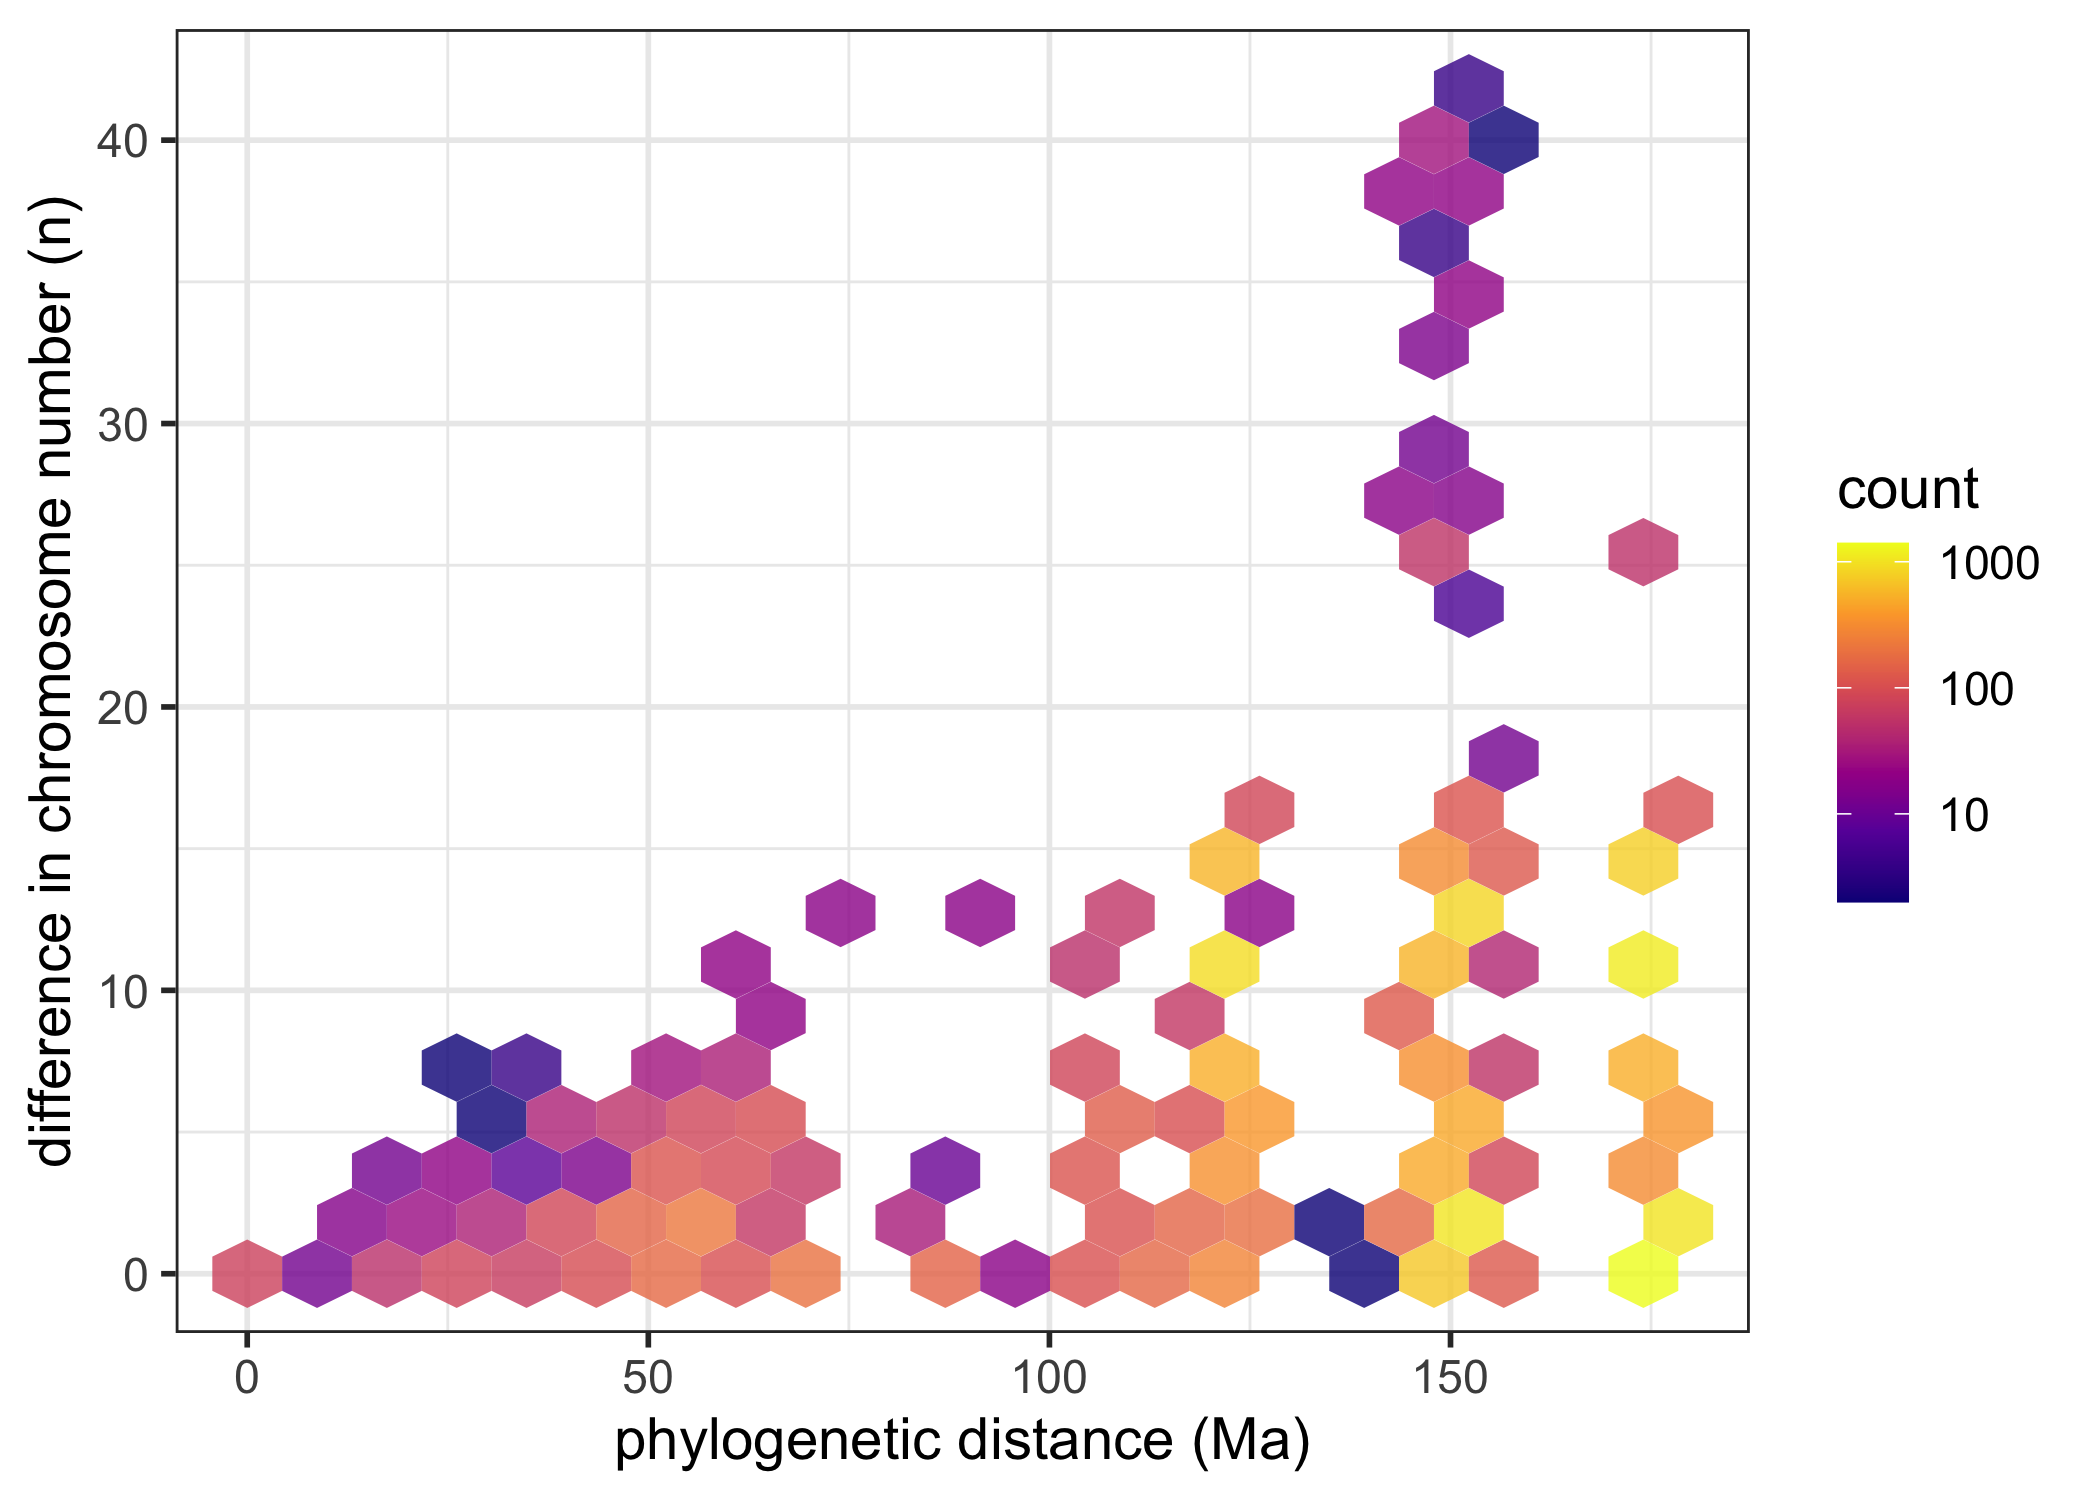
\includegraphics[width = \linewidth]{figures/taxon-pairs-distances.png}
  \caption{Phylogenetic distance (in millions of years) in relation to differences in chromosome numbers (2n) for each pair of taxa in the chameleon tree. Note that the cluster of values with chromosome differences greater than 10 are comparisons of various taxa with \textit{Rieppeleon kerstenii} (2n = 62).
}
  \label{fig-otus-pairwise}
\end{figure} 

% figure
\newpage
\begin{figure}[H]
 \centering
  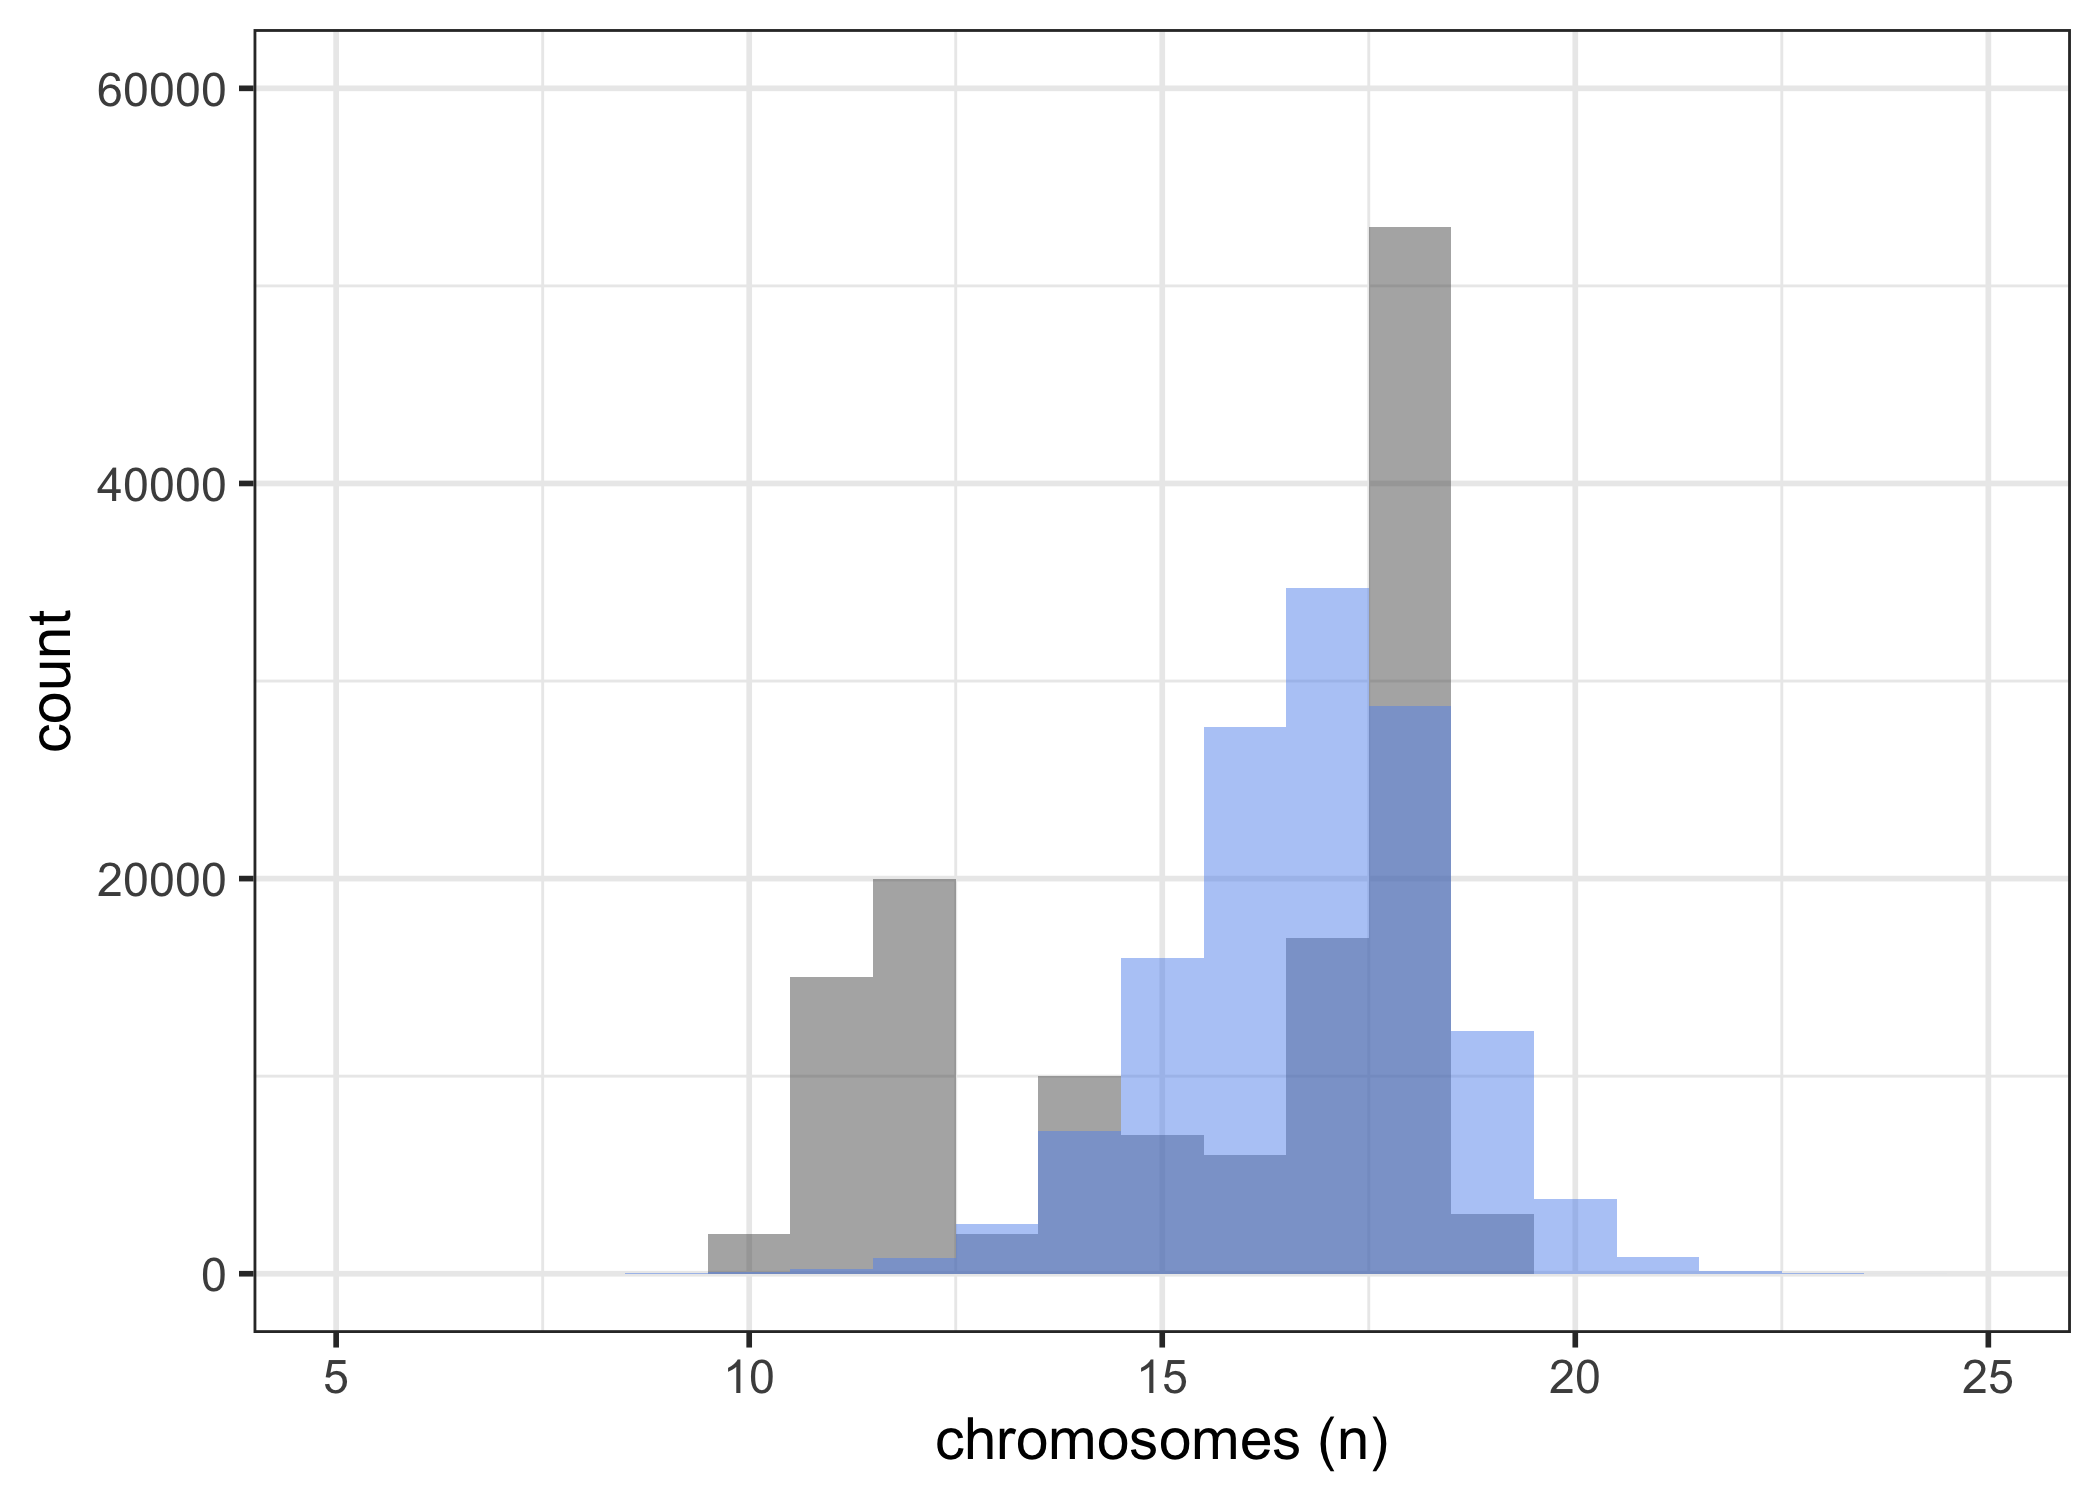
\includegraphics[width = \linewidth]{figures/chromevol-simulations-numbers.png}
  \caption{Distribution of observed (grey) and predicted (blue) haploid numbers of chromosomes in chameleons, excluding \textit{Rieppeleon kerstenii}. Predicted values are based on 1,000 simulations using the optimised parameters taken from the best fitting model identified in the chromosome evolution analyses above (Constant Rates, removing \textit{Rieppeleon kerstenii}, and using n = 18 as the root node). Observed values were multiplied by 1,000 to aid comparisons.
}
  \label{fig-otus-predicted}
\end{figure} 

%-------------------
\newpage
\section{Correlations among haploid chromosome number (n) chromosome morphology}

% figure
\begin{figure}[H]
 \centering
  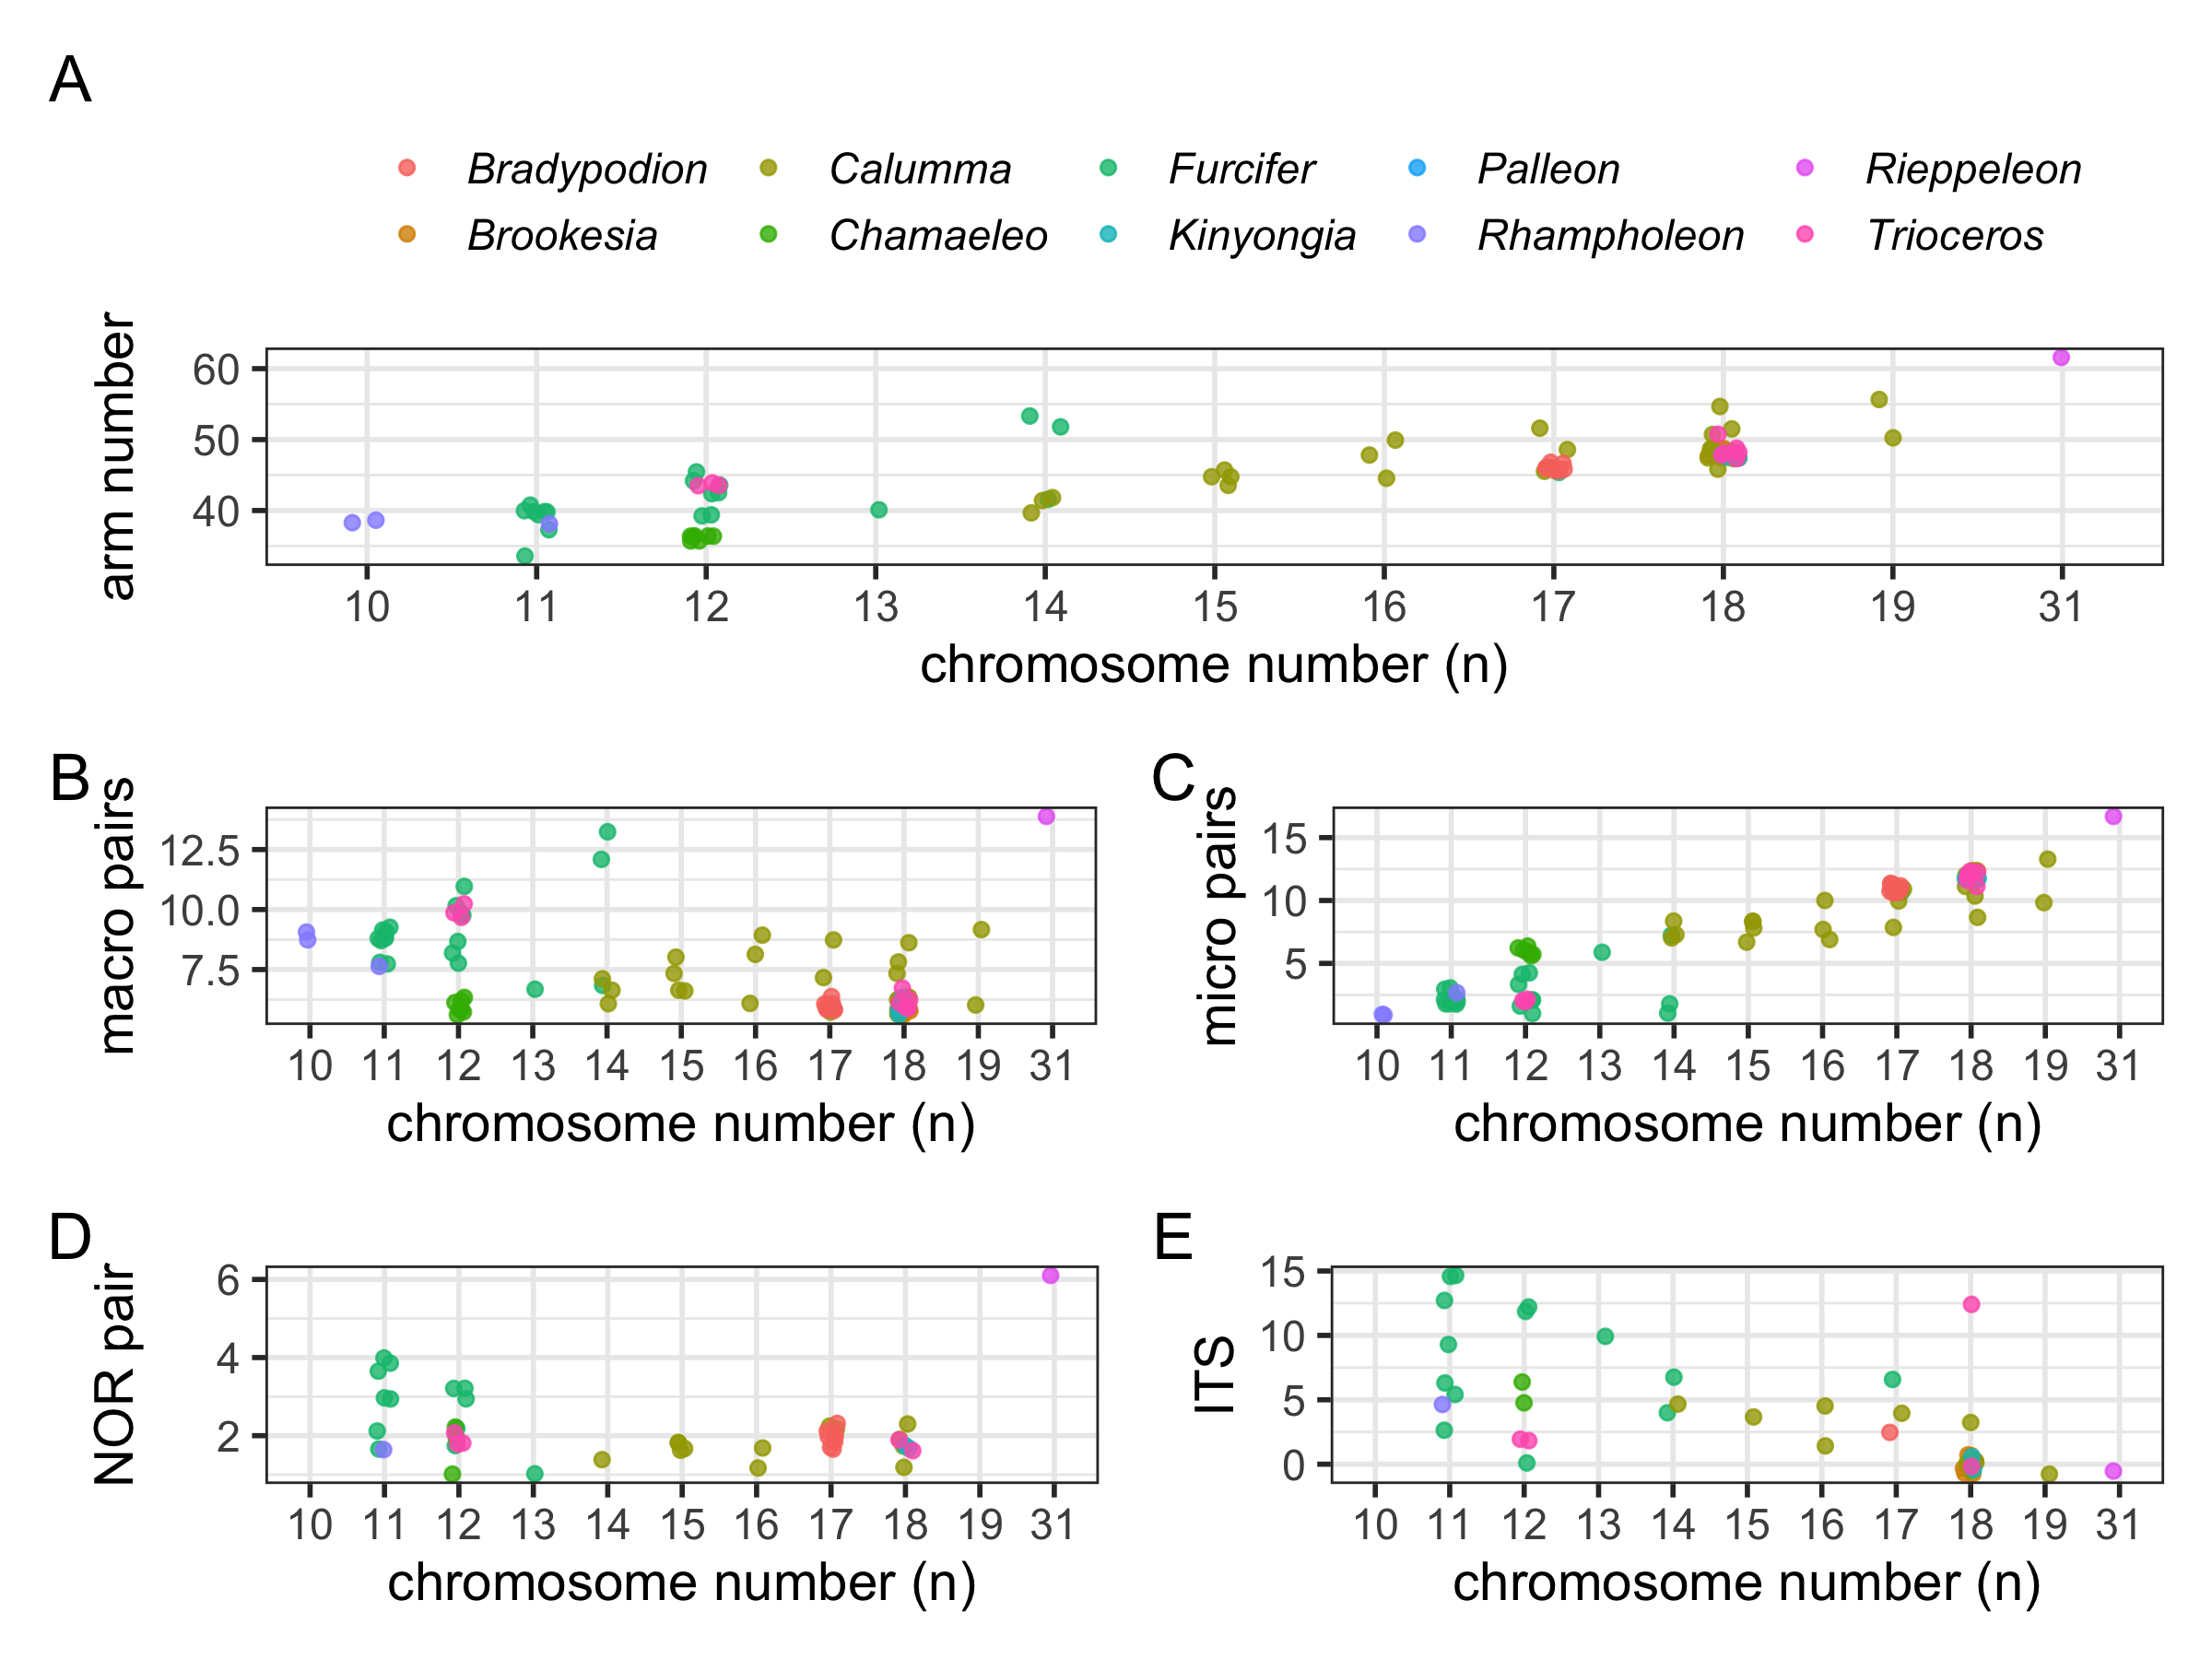
\includegraphics[width = \linewidth]{figures/morphology-chromono.png}
  \caption{Correlations among haploid chromosome number (n) and various morphological features of chromosomes including A) arm number; B) macrochromosome pairs; C) number of microchromosome pairs; D) position of NOR loci; and E) number of interstitial telomeric sequences (ITS). Colours indicate genera.
}
  \label{fig-morph}
\end{figure} 

%-------------------------------------------------------------------------------
\newpage
\section{Calibration points for phylogeny}
%-------------------------------------------------------------------------------

Please note that our constraints differ from those used by Tolley \textit{et al.}\cite{tolley2013large}. Given that (accurately identified) fossils (with apomorphies) provide hard minima for the emergence of clades we consider conservative constraints to be constraints with shallower dates.
 
\subsection{External points}
 
\subsubsection*{Node 1. (Lepidosauria) – 250 Ma}
For Lepidosauria we used a point fix of 250 Ma. Note that this node by definition also applies to both total-group Squamata and total-group Rhynchocephalia\cite{evans2003feet}. The oldest known fossil material representing total-group Squamata is currently considered to be \textit{Megachirella wachtleri} from the Anisian of Italy\cite{renesto2003new,simoes2018origin}. If this taxon is indeed a stem squamate it provides a hard minimum of 242 Ma for total group Squamata and thus also Lepidosauria. The oldest known fossil material representing total group Rhynchocephalia is not much younger (238-240 Ma within the Ladinian) and is represented by partial skull and jaw bones from the Ladinian of Germany\cite{jones2013integration,schoch2018tetrapod}. This material has not been fully described but may include at least three different genera which shows that Rhynchocephalia must have diversified by this time. Fossils representing likely stem lepidosaurs (e.g. \textit{Sophineta}, \textit{Fraxinisaura}) are known from the Early and Middle Triassic\cite{evans2009small,schoch2018tetrapod}. Previous molecular divergence estimates for Lepidosauria have differed greatly\cite{jones2013integration} with median estimates as deep as the Early Permian (e.g. 281 Ma) and as shallow as the Late Triassic (e.g. 227 Ma) and associated confidence intervals can exceed 20 million years. Estimates shallower than the Middle Triassic can be rejected with empirical evidence from the fossil record\cite{jones2013integration,simoes2018origin}. Much older origin times deep within the Permian are possible (e.g.\cite{simoes2018origin}) but there are currently no convincing crown-group lepidosaurs known from this time period. Overall, a divergence date near the Permian-Triassic boundary seems appropriate.  

\subsubsection*{Node S (Squamata) – not constrained}
We did not constrain the node for crown-group Squamata. For the origin and divergence of crown group Squamata, molecular analyses have suggested a wide range of possible dates spanning the Permian, Triassic, and Jurassic (see\cite{jones2013integration}). However, several analysis provide a median estimate that is within 15 Ma of the Triassic-Jurassic boundary\cite{jones2013integration,simoes2018origin,burbrink2020interrogating}. The early history of crown-group lizards is poorly known but fossil material is known from the Middle Jurassic (e.g.\cite{evans1998crown,evans2003feet,evans2008skull}). Available evidence suggests that the origin for crown-group Squamata lies near the Triassic-Jurassic boundary. 

\subsubsection*{Node U. (Unidentata) – not constrained}
We did not constrain the node for crown group Unidentata.
 
\subsubsection*{Node 2. (Xantusia-Cordylus) – 62.5 Ma (min) 100 Ma (max)}
We constrain the divergence between cordylids and xantusiids to 61 Ma based on \textit{Palaeoxantusia fera} from the Palaeocene rocks of the Gidley and Silberling quarries of USA\cite{hecht1956new,sullivan1991paleocene}. The material exhibits several traits suggestive of a close affinity to xantusiids\cite{smith2009eocene,smith2011long}. The Gidley and Silberling rocks are suspected to be correlated with magnetic polarity chron C27r\cite{butler1987magnetic} now inferred to be 63.5 and 62.5 Mya\cite{gradstein2012geologic,dinares2014astronomical,ogg2020geomagnetic}. Therefore, we apply a hard minimum of 62.5 Ma.

\subsubsection*{Node 3. (Laterata) – 138.7 Ma (min) 140.1 (max)}
The node defining Laterata (Teiioidea, Amphisbaenia, and Lacertidae) was constrained to 138.7 Ma. The oldest known fossil material that can be referred to Lacertidae or Teiiodea is \textit{Purbicella ragei} from the Cherty Freshwater Beds of the Lulworth Formation of the Purbeck Group, England UK\cite{evans2012new}. Key morphological characters present in the material include the presence of a pterygoid lappet on the quadrate, a narrow pyriform recess, a jugal located dorsal to the maxilla, and a parietal with anterior tabs that slot into the underside of the frontal\cite{conrad2008phylogeny,evans2008skull}. The Cherty Freshwater Beds are part of the Purbeck Group and considered to be Berriasian in age, Lower Cretaceous\cite{radley2012wealden}. The upper boundary of the Berriasian is considered to be 139.4 $\pm$ 0.7 Ma\cite{gradstein2012geologic} therefore, providing a hard minimum of 138.7. This constraint is older than the date of 122 $\pm$ 1.0 Ma based on \textit{Ptilodon}\cite{nydam2002lizards,winkler1990early} used in Tolley \textit{et al.}\cite{tolley2013large}.
  
\subsubsection*{Node 4. (Lacertibaenia) – 61 Ma (min) 100 (max)}
We constrain the node representing the divergence of Lacertibaenia (Amphisbaenia and Lacertidae) to 61 Ma based on \textit{Plesiorhineura tsentasi} from the Palaeocene of USA\cite{sullivan1985new}. Older fossil material named \textit{Hodzhakulia} (112 $\pm$ 1.0 Ma) used in Tolley \textit{et al.}\cite{tolley2013large} is less certainly amphisbaenian and may therefore be a problematic calibration point\cite{hipsley2009integration}.
 
\subsubsection*{Node 5. (Anguimorpha) – 148 Ma (min) 155 Ma (max)}
Anguimorpha 148 Ma, minimum hard bound based on \textit{Dorsetisaurus} sp. from the Late Jurassic Morrison Formation of North America\cite{prothero1980late,evans1999upper,conrad2008phylogeny,jones2013integration}. Combined evidence analysis places \textit{Dorsetisaurus purbeckensis} as a non-anguiform anguimorph and therefore the oldest known representative of Anguimorpha\cite{conrad2011combined}.
 
\subsubsection*{Node 6. (crown Serpentes) – 93.9 Ma (min) 100.5 Ma (max)}
The divergence between \textit{Liotyphlops} and \textit{Dinodon} (crown Serpentes) was constrained to a hard minimum of 93.9 Ma and maximum of 100.5 Ma based on \textit{Haasiophis terrasanctus} from the Late Cretaceous of the Middle East\cite{tchernov2000fossil,rieppel2003anatomy}. This date is the same as used elsewhere (e.g. 93.9 Ma used by\cite{head2015fossil,hsiang2015origin})
 
\subsubsection*{Node G. (Iguania) – not constrained}
The oldest stem iguanians are uncertain\cite{bolet2013fossil}. Fossils from the Early Jurassic previously referred to iguanians\cite{evans2002fossil} may belong to another clade (e.g.\cite{jones2013integration}).
 
\subsubsection*{Node 7. (Anguioidea) – 74.5 Ma (min) 76.6 (max)}
The node representing the most recent common ancestor (MRCA) of Xenosauridae and Anguidae was constrained to a minimum of 74.5 Ma. The oldest known fossil material representing Anguidae is \textit{Odaxosaurus}\cite{nydam2013lizards} from the Kaiparowits Formation, locality OMNH V5, of Garfield County, Utah, USA. An integrated analysis using morphological and molecular data recovers \textit{Odaxosaurus piger} as the sister taxon to Glyptosaurinae\cite{conrad2011combined}. Extensive stratigraphic and isotope analyses of the Kaiparowits Formation indicate an age range of 74.5 - 76.6 Ma\cite{roberts200540ar,roberts2013kaiparowits}. Therefore providing a hard minimum estimate of 74.5 Ma. 
 
\subsubsection*{Node 8. (Pleurodonta) – 70 Ma (min) 71.2 (max)}
Crown-group pleurodont Iguania is constrained to a minimum date of 70 Ma. The earliest certain representative of crown-group pleurodont iguanians is \textit{Saichangurvel}\cite{conrad2007complete} from the Late Campanian (72.5 $\pm$ 2.5 Ma) of Mongolia. This constraint was also used by Tolley \textit{et al.}\cite{tolley2013large} with a date of 70.6 $\pm$ 0.6 Ma.
 
\subsection{Internal points}
\subsubsection*{Node C. (stem Chamaeleonidae) – not constrained}
We do not constrain this node. Although a fossil skeleton (specimen JZC Bu154) from the Cretaceous of Myanmar (99 Ma) has been referred to the stem of Chamaeleonidae\cite{daza2016mid}, and previously used to constrain molecular divergence analyses (e.g.\cite{skawinski2017evolution}), this material represents an abanerpetontid and is not even a lepidosaur\cite{daza2020enigmatic}.
 
\subsubsection*{Node 9. (\textit{Calumma}) – 16 Ma (min) 20 Ma (max)}
The genus \textit{Calumma} is constrained to a hard minimum date of 16 Ma. The earliest known representative of this genus is a nearly complete articulated skull, \textit{Calumma benovskyi}, from the Early Miocene Hiwegi Formation of Rusinga Island Kenya\cite{vcervnansky2020only}. Detailed morphological comparisons and phylogenetic analyses confidently place this specimen within \textit{Calumma}\cite{vcervnansky2020only}.
 
\subsubsection*{Node 10. (\textit{Chamaeleo}) – 16.6 Ma (min) 20 Ma (max)}
The genus \textit{Chamaeleo} is constrained to a minimum date of 16.6 Ma. The earliest known representatives of this genus come from units referred to the 3 to 6 mammal Neogene zones (MN)\cite{vcervnansky2010revision,bolet2013fossil}. Zone 3 corresponds to approximately 16.6 to 20 Ma and therefore provides a hard minimum date of 16.6.\cite{van2011biostratigraphy}. The origin maybe older but we prefer to use the shallower data so that the error is more certainly unidirectional.

%-------------------------------------------------------------------------------
% Samples
%-------------------------------------------------------------------------------
\newpage
\section{List of samples}

A full list of samples used in the analyses is listed in Table \ref{table-samples}.

% Table samples
\begin{longtable}{llll}

\caption{Complete list of samples used in the molecular and cytogenetic analyses}\\ 
  
\hline

\textbf{species} & \textbf{sample ID} & \textbf{sex} & \textbf{locality} \\

\hline

\textit{Brookesia ambreensis} & GA303 & F & An'Ala\\
\textit{Brookesia ambreensis} & GA304 & M & An'Ala\\
\textit{Brookesia betschi} & GAA1 & M & Marojejy\\
\textit{Brookesia betschi} & GAA2 & F & Marojejy\\
\textit{Brookesia brygooi} & FAZC11696 & F & Anosibe An'Ala\\
\textit{Brookesia brygooi} & FAZC11697 & F & Ambolokopatrika\\
\textit{Brookesia decaryi} & GA392 & M & Ambolokopatrika\\
\textit{Brookesia decaryi} & FAZC11609 & F & Ambolokopatrika\\
\textit{Brookesia dentata} & GA309 & F & Mandraka\\
\textit{Brookesia ramanantsoai} & GA709 & F & Beparasy\\
\textit{Brookesia ramanantsoai} & GA710 & F & Beparasy\\
\textit{Brookesia stumpffi} & GAB1 & M & Manongarivo\\
\textit{Brookesia stumpffi} & GA7 & F & Manongarivo\\
\textit{Brookesia superciliaris} clade 2 & GA199 & F & Fiherenana\\
\textit{Brookesia superciliaris} clade 2 & GAA3 & M & Fiherenana\\
\textit{Brookesia superciliaris} clade 1 & GA583 & M & Moramanga\\
\textit{Brookesia superciliaris} clade 1 & FAZC11604 & M & Anosibe An'Ala\\
\textit{Brookesia therezieni} & FGMV983 & M & Andasibe\\
\textit{Brookesia therezieni} & FGMV985 & F & Andasibe\\
\textit{Brookesia thieli} clade 2 & GA89 & F & Vohidrazana\\
\textit{Brookesia thieli} clade 2 & GA40 & M & Vohidrazana\\
\textit{Brookesia thieli} clade 2 & GA584 & F & Moramanga\\
\textit{Brookesia thieli} clade 2 & GA706 & F & Beparasy\\
\textit{Brookesia tuberculata} & FGMV3088 & F & Montagne D'Ambre\\
\hline
\textit{Calumma amber} & FGMV3126 & NA & NA\\
\textit{Calumma amber} & FGMV3134 & NA & NA\\
\textit{Calumma ambreense} & FGMV3121 & NA & Montagne D'Ambre\\
\textit{Calumma ambreense} & FGMV3123 & NA & Montagne D'Ambre\\
\textit{Calumma brevicorne} clade 2 & FAZC11778 & M & Fiherenana\\
\textit{Calumma brevicorne} clade 2 & FAZC11779 & F & Fiherenana\\
\textit{Calumma brevicorne} clade 1 & GA594 & F & Mandraka\\
\textit{Calumma brevicorne} clade 1 & GA48 & F & Mandraka\\
\textit{Calumma crypticum} & GA404 & M & Ranomafana\\
\textit{Calumma cucullatum} & FAZC7633 & M & Ambatolaidama\\
\textit{Calumma emelinae} & GA310 & F & Fiherenana\\
\textit{Calumma emelinae} & GA314 & F & Fiherenana\\
\textit{Calumma fallax} clade 1 & GA382 & M & Ranomafana\\
\textit{Calumma fallax} clade 1 & GA365 & F & Ranomafana\\
\textit{Calumma fallax} clade 2 & GA494 & F & Mandraka\\
\textit{Calumma fallax} clade 2 & GA495 & F & Mandraka\\
\textit{Calumma furcifer} & GA311 & F & Fiherenana\\
\textit{Calumma gallus} clade 1 & ZCMV601 & F & An'Ala\\
\textit{Calumma gallus} clade 1 & ZCMV602 & F & An'Ala\\
\textit{Calumma gallus} clade 2 & GA763 & F & An'Ala\\
\textit{Calumma gallus} clade 2 & GA763 & F & An'Ala\\
\textit{Calumma gallus} clade 3 & FGMV642 & F & Ambohitsara\\
\textit{Calumma gastrotaenia} clade 2 & GA368 & F & Ranomafana\\
\textit{Calumma gastrotaenia} clade 2 & GA557 & F & Moramanga\\
\textit{Calumma gastrotaenia} clade 1 & FGMV3043 & NA & Vohidrazana\\
\textit{Calumma gastrotaenia} clade 1 & GA87 & F & Andasibe\\
\textit{Calumma glawi} & GA364 & F & Ranomafana\\
\textit{Calumma globifer} & GA501 & F & Mandraka\\
\textit{Calumma globifer} & FAZC11776 & NA & Mandraka\\
\textit{Calumma hilleniusi} & FAZC12265 & F & Ambositra\\
\textit{Calumma malthe} & GA312 & F & Fiherenana\\
\textit{Calumma malthe} & GA963 & M & Ambatolaidama\\
\textit{Calumma nasutum} & FGMV984 & M & Andasibe\\
\textit{Calumma nasutum} & FGMV985 & F & Andasibe\\
\textit{Calumma oshaughnessyi} & GA383 & NA & Ranomafana\\
\textit{Calumma oshaughnessyi} & GA453 & F & Ranomafana\\
\textit{Calumma parsonii} & FGMV3118 & NA & Vohidrazana\\
\textit{Calumma radamanus} & GA236 & F & Torotofuzi\\
\textit{Calumma} sp. 1 & GA429 & M & Ranomafana\\
\textit{Calumma} sp. 1 & GA430 & F & Ranomafana\\
\textit{Calumma} sp. 2 & FGMV3125 & NA & NA\\
\textit{Calumma} sp. 3 & GA45 & M & Mandraka\\
\textit{Calumma} sp. 3 & GA46 & M & Mandraka\\
\textit{Calumma} sp. 4 & GA558 & M & Moramanga\\
\textit{Calumma tarzan} & FAZC12208 & M & Benava\\
\hline
\textit{Furcifer belalandensis} & GA379 & F & Ranomafana\\
\textit{Furcifer belalandensis} & FGMV647 & M & Ifanadiana\\
\textit{Furcifer belalandensis} & GA465 & F & Belalanda\\
\textit{Furcifer campani} & GA104 & F & Tsiafajavona\\
\textit{Furcifer campani} & GA105 & F & Tsiafajavona\\
\textit{Furcifer labordi} & GA331 & M & Marofandilia\\
\textit{Furcifer labordi} & GA332 & F & Marofandilia\\
\textit{Furcifer lateralis} & FAZC11278 & M & Antoetra\\
\textit{Furcifer lateralis} & FAZC11279 & F & Antoetra\\
\textit{Furcifer major} & GA456 & F & Belalanda\\
\textit{Furcifer minor} & GA489 & F & Antoetra\\
\textit{Furcifer nicosiai} & GA81 & F & Isalo\\
\textit{Furcifer nicosiai} & FGMV1476 & NA & Analalava\\
\textit{Furcifer pardalis} & FGMV2241 & M & Tanatava\\
\textit{Furcifer pardalis} & FAZC12269 & F & Tanatava\\
\textit{Furcifer petteri} & FGMV3015 & F & Montagne D'Ambre\\
\textit{Furcifer petteri} & FGMV3016 & M & Montagne D'Ambre\\
\textit{Furcifer rhinoceratus} & GA490 & F & Antoetra\\
\textit{Furcifer verrucosus clade 2} & GA15 & M & Tulear\\
\textit{Furcifer verrucosus clade 2} & GA440 & F & Tulear\\
\textit{Furcifer verrucosus clade 1} & GA581 & F & South of Antoetra\\
\textit{Furcifer verrucosus clade 1} & GA582 & F & South of Antoetra\\
\textit{Furcifer viridis} & GA513 & F & Mandrivazo\\
\textit{Furcifer viridis} & GA516 & M & Mandrivazo\\
\textit{Furcifer wilsii} & GA174 & F & Fiherenana\\
\textit{Furcifer wilsii} & GA175 & M & Fiherenana\\
\hline
\textit{Palleon nasus} & GA445 & M & Marofandilia\\
\textit{Palleon nasus} & GA363 & M & Marofandilia\\
\hline

\label{table-samples}
\end{longtable}


%-------------------------------------------------------------------------------
% Cytogenetic analyses
%-------------------------------------------------------------------------------
\newpage
\section{Cytogenetic results}
Standard karyotyping was successfully performed on all the considered species (n = 54) but \textit{Calumma cucullatum} and \textit{Calumma} sp. 4, which did not provide suitable metaphase plates.
Considering the quality and number of metaphase plates, Ag-NOR staining was performed on all the \textit{Brookesia} and \textit{Palleon} species here considered, 13 \textit{Calumma} species and 11 \textit{Furcifer} species. 
Similarly, TELO-FISH was successfully performed on nine \textit{Brookesia}, 13 \textit{Calumma} and 12 \textit{Furcifer} species, respectively (see Figures \ref{fig-s1} - \ref{fig-s6}).
Chromosome number was found to be constant (2n = 36, AN = 48) in all the \textit{Brookesia} species (n = 13) and in \textit{Palleon nasus} (Figure \ref{fig-s1}), and invariably with six macro- and 12 micro-chromosome pairs.

\noindent All the macrochromosome pairs resulted metacentric with the only exception of the 2nd submetacentric pair in \textit{P. nasus}. 
No heteromorphic chromosome pairs were found in any \textit{Brookesia} species or in \textit{P. nasus}.
No ITS signals were found in the karyotype of any \textit{Brookesia} species or in \textit{P. nasus} (Figure \ref{fig-s2}).

\noindent In the genus \textit{Calumma}, karyotypes varied from 2n = 38 (in \textit{C. tarzan} and \textit{C. amber}) to 2n = 28 (in \textit{C. nasutum} and \textit{C. fallax} clade 2) (AN = 40-56), with 2n = 36 resulting the most common chromosome configuration in the genus (in 10 out of 24 species studied; Figure \ref{fig-s3}). 
Karyotype of 2n = 34, 32 and 30 chromosomes were showed by four, three and four species, respectively. 
A variable number of macro- (6-9) and micro-chromosome pairs (7-13) was also recorded among the studied species of the genus. 
Chromosome morphology is also variable in \textit{Calumma}, macrochromosome pairs are generally biarmed (from meta- to sub-telocentric pairs), but telocentric elements were observed in \textit{Calumma} sp. 1 (7th pair). 

\noindent A heteromorphic pair was observed in the karyotype of \textit{C. crypticum}. 
NOR bearing pairs were detected in 14 species, on the 1st (three species) or 2nd chromosome pair (11 species). 
ITS signals (n = 2-4) were found in six species showing karyotypes from 2n = 36 to 2n = 28 (Figure \ref{fig-s4}).

\noindent The genus \textit{Furcifer} showed karyotypes ranging from 2n = 34 (only in \textit{F. balteatus}) to 2n = 22 (the most common karyotype configuration in the genus, found in eight out of 16 species studied; AN = 34-54; Figure \ref{fig-s5}). 
Karyotypes of 2n = 28 were showed by two species (\textit{F. wilsii} and \textit{F. labordi}), 2n = 26 by one species (\textit{F. campani}) and 2n = 24 by five species. 

\noindent Macrochromosome pairs ranged from six to 13 pairs, while microchromosomes from one to 11 pairs. 
Chromosome morphology is mostly biarmed in the genus (meta- and submeta-centric pairs are common in the genus), but 1-2 telocentric pairs are present in the karyotype of \textit{F. belalandensis} and \textit{F. minor}.
Heteromorphic chromosome pairs were found in seven species, usually on the last macrochromosome pair. 
In the species analysed here, loci of NOR are always on macrochromosomes (1st, 2nd, 3rd or 4th pair). 
A highly variable number of ITS signals (n = 2-14) were found in 11 species with 2n = 34-22 (Figure \ref{fig-s6}).

% figures are large so give them a page each
\newpage
% figure marcello s1
\begin{figure}[H]
 \centering
  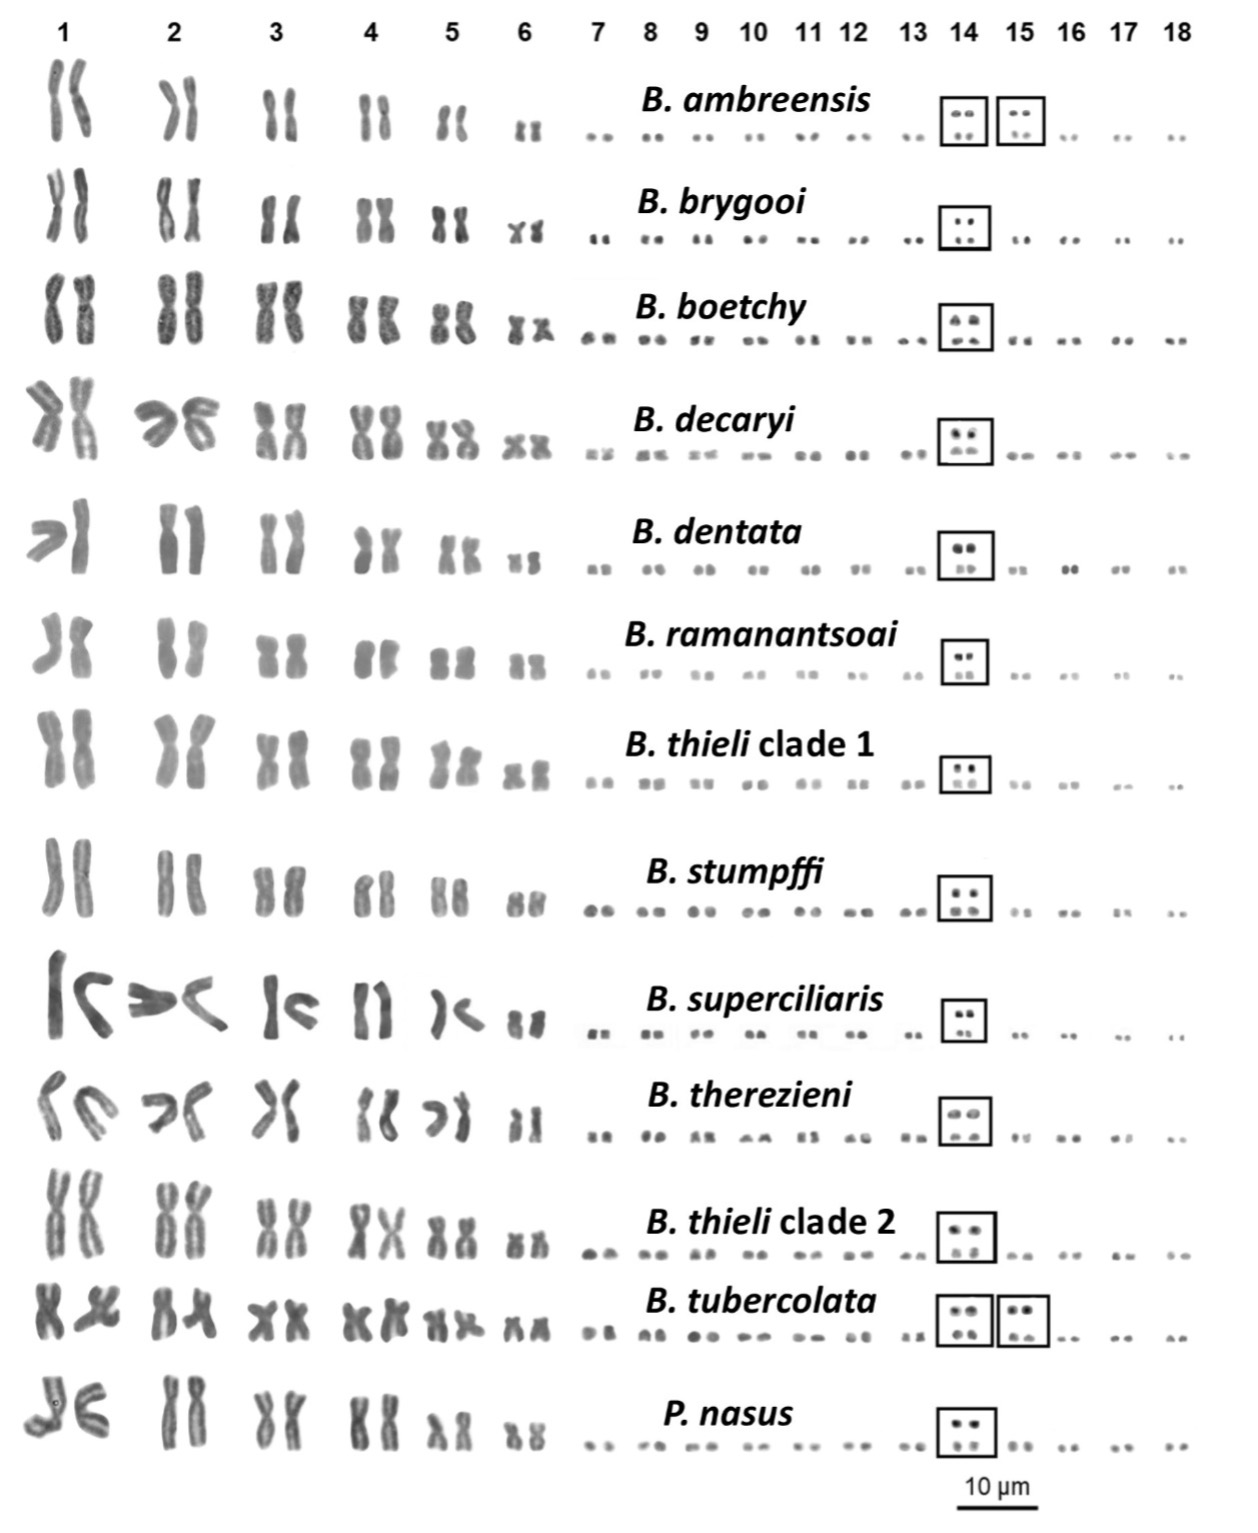
\includegraphics[width = \linewidth]{figures/marcello-s1.jpg}
  \caption{Karyotypes of \textit{Brookesia} and \textit{Palleon} stained with Giemsa. Squares highlight the NOR-bearing chromosome pairs stained with Giemsa (left) and Ag-NOR (right).
}
  \label{fig-s1}
\end{figure}

\newpage
% marcello figure s2
\begin{figure}[H]
 \centering
  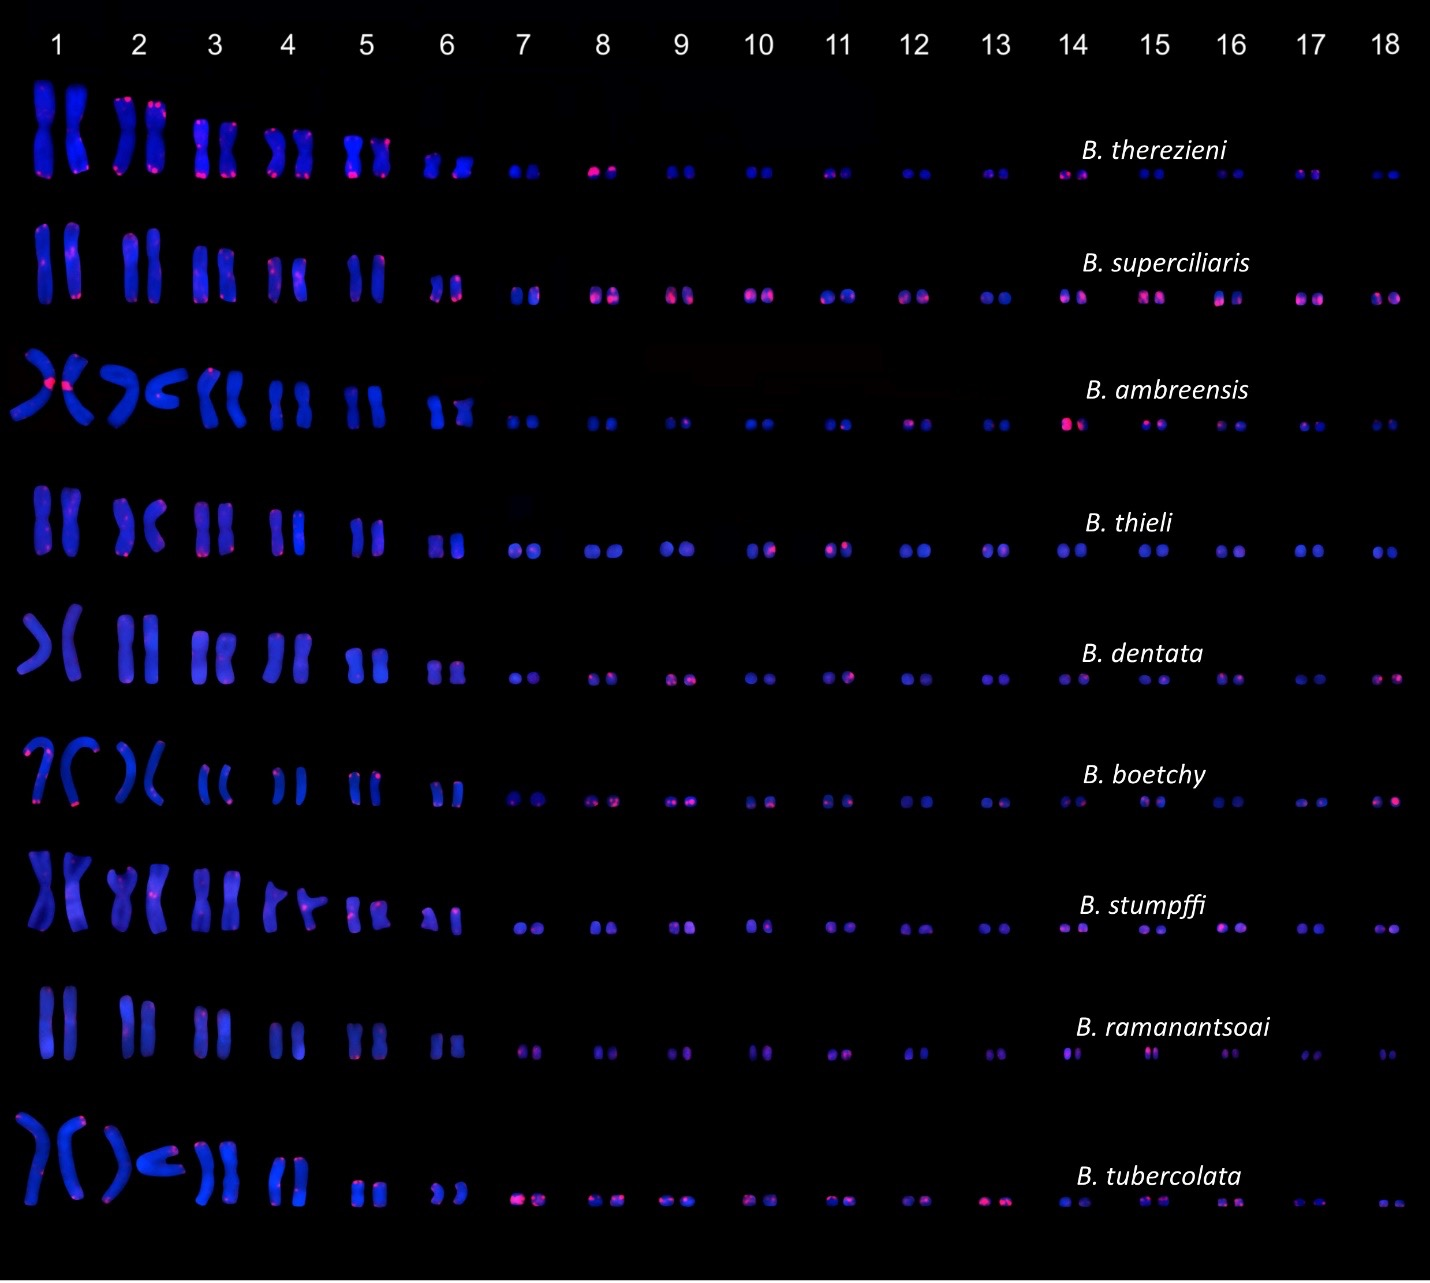
\includegraphics[width = \linewidth]{figures/marcello-s2.jpg}
  \caption{Karyotypes of \textit{Brookesia} and \textit{Palleon} stained with TELO-FISH.
}
  \label{fig-s2}
\end{figure}

\newpage
% marcello figure s3
\begin{figure}[H]
 \centering
  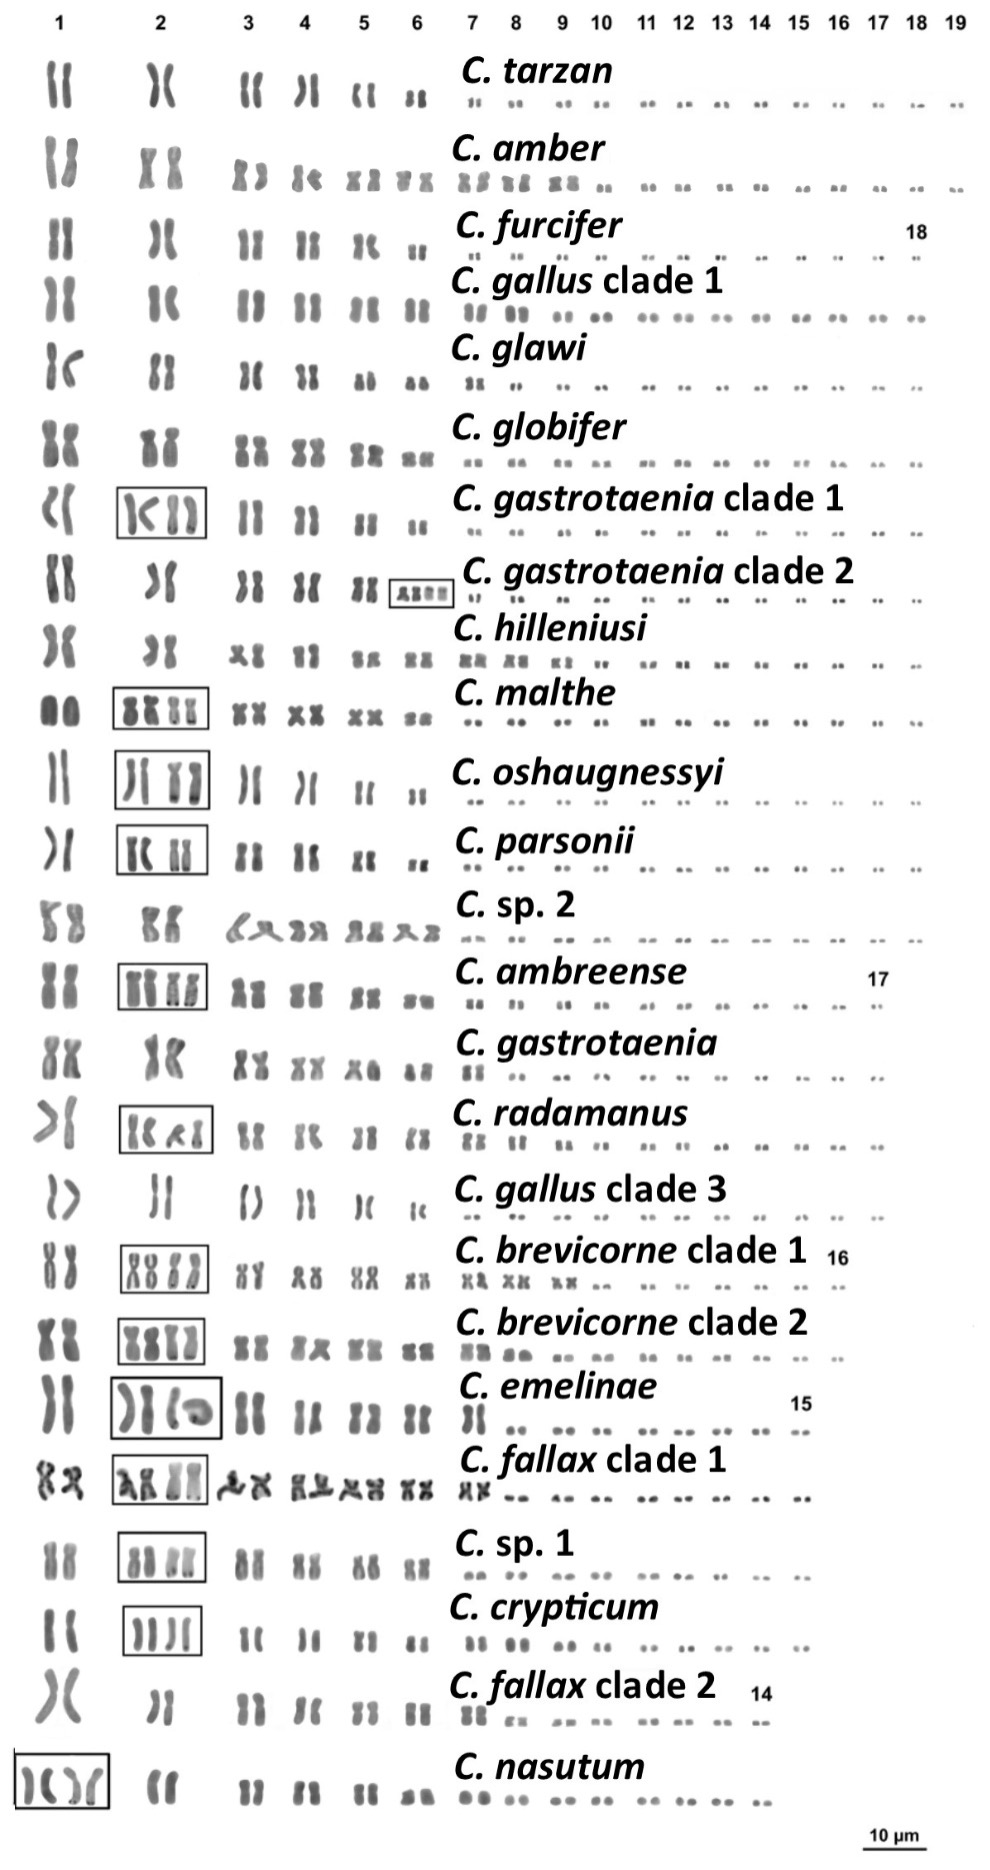
\includegraphics[width = 0.8\linewidth]{figures/marcello-s3.jpg}
  \caption{Karyotypes of \textit{Calumma} stained with Giemsa. Squares highlight the NOR-bearing chromosome pairs stained with Giemsa (left) and Ag-NOR (right).
}
  \label{fig-s3}
\end{figure}

\newpage
% marcello fig-s4
\begin{figure}[H]
 \centering
  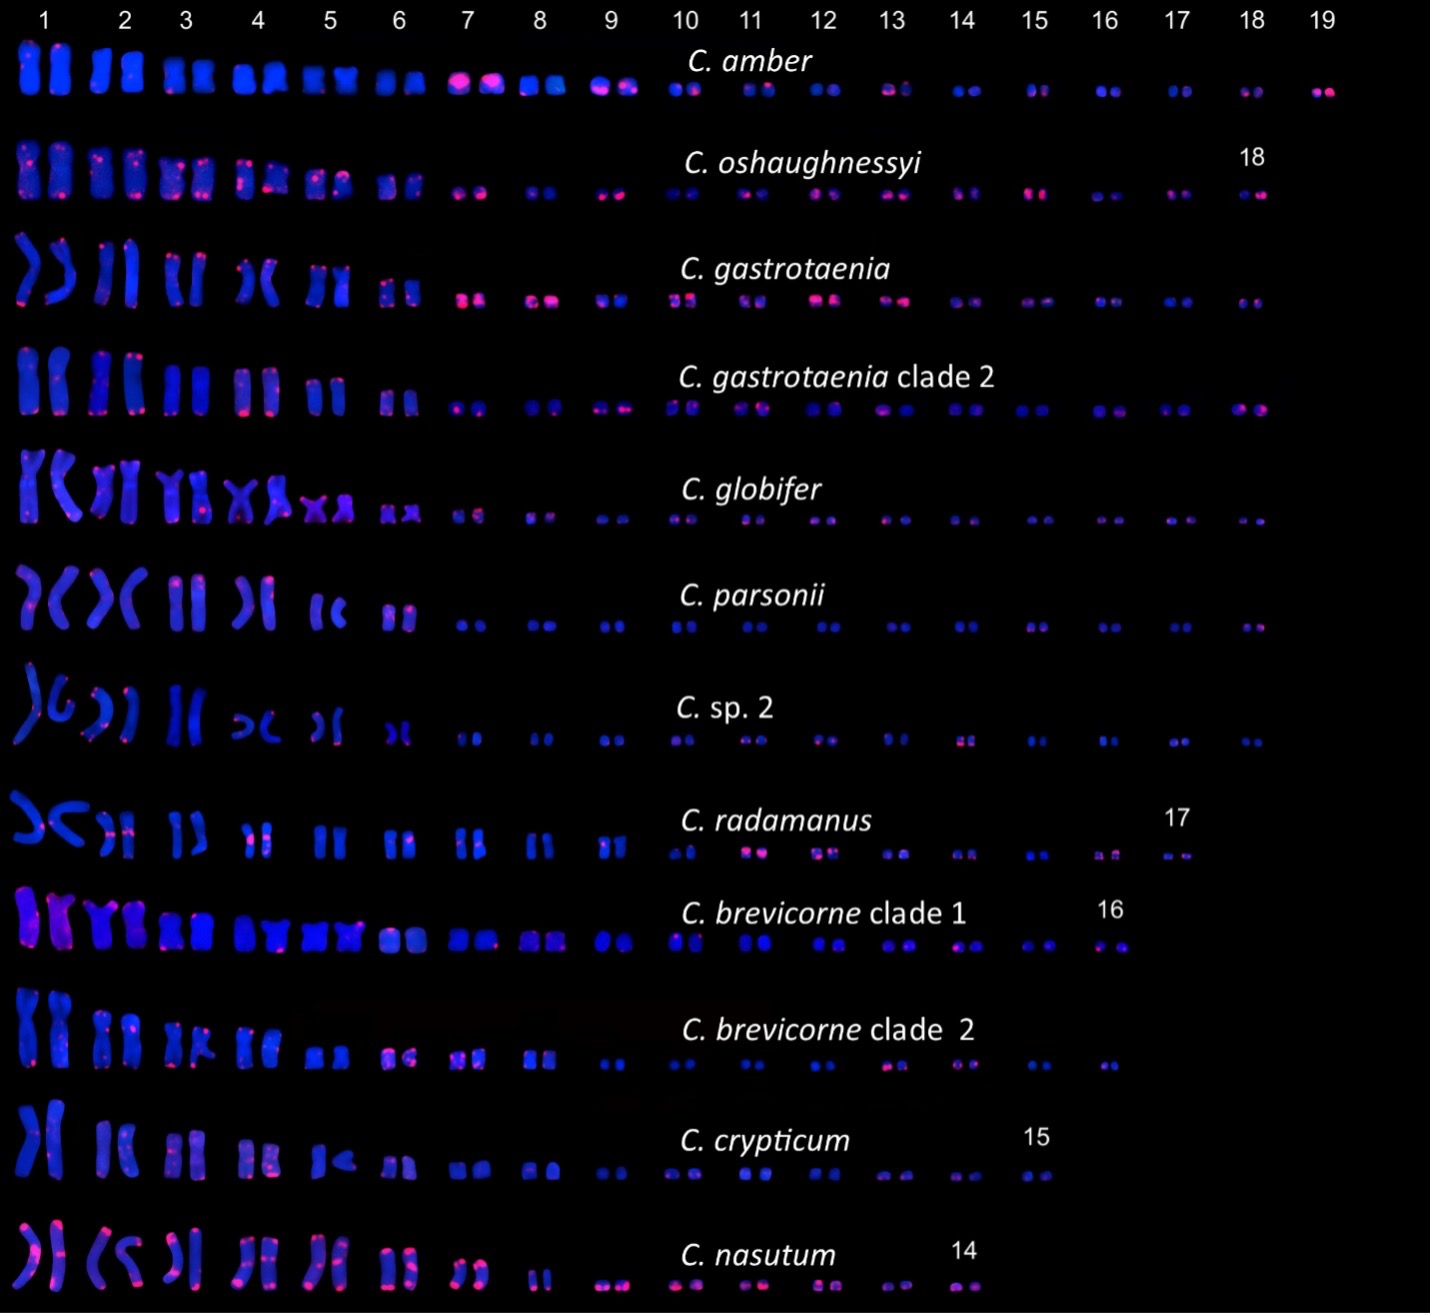
\includegraphics[width = \linewidth]{figures/marcello-s4.jpg}
  \caption{Karyotypes of \textit{Calumma} stained with TELO-FISH.
}
  \label{fig-s4}
\end{figure}

\newpage
% marcello figure s5
\begin{figure}[H]
 \centering
  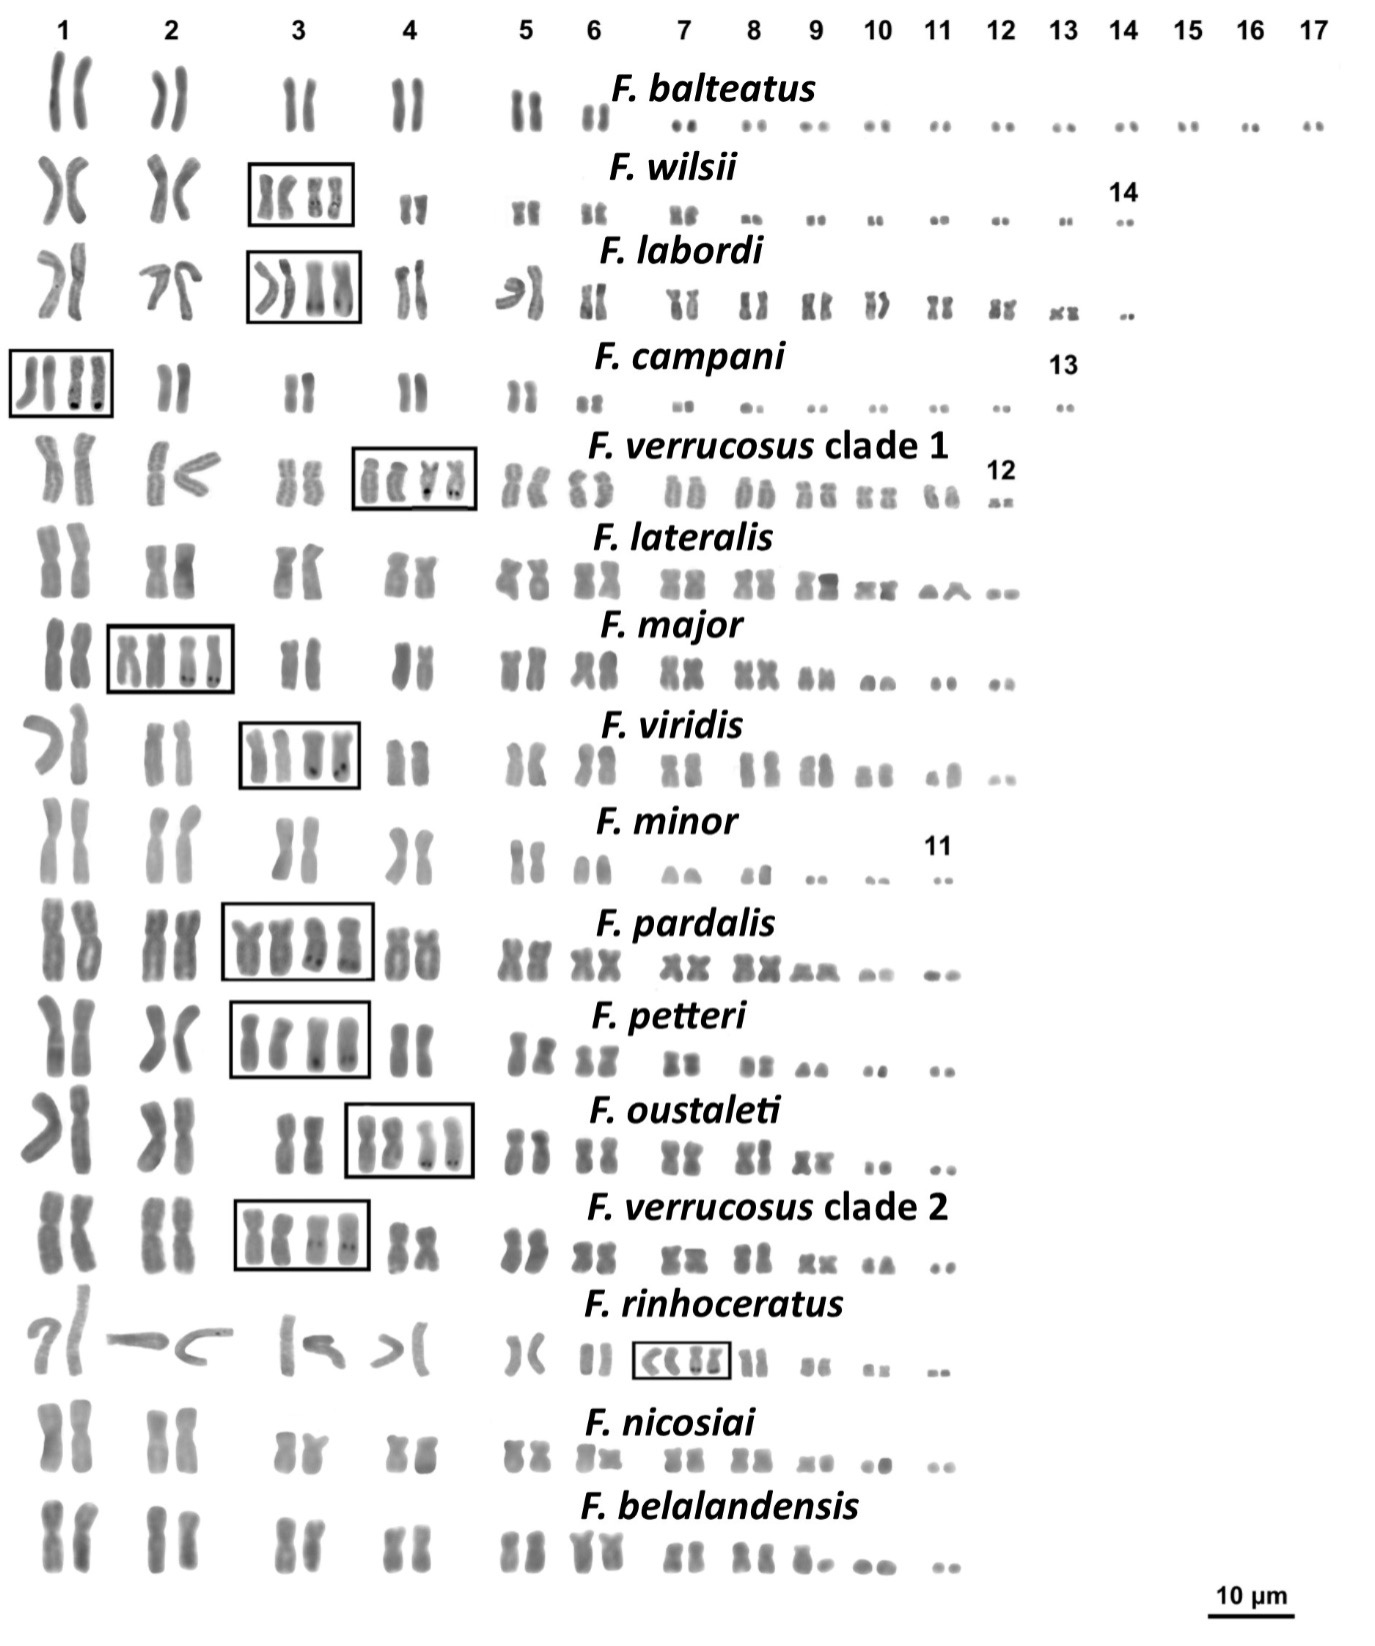
\includegraphics[width = \linewidth]{figures/marcello-s5.jpg}
  \caption{Karyotypes of \textit{Furcifer} stained with Giemsa. Squares highlight the NOR-bearing chromosome pairs stained with Giemsa (left) and Ag-NOR (right).
}
  \label{fig-s5}
\end{figure}

\newpage
% marcello fig-s6
\begin{figure}[H]
 \centering
  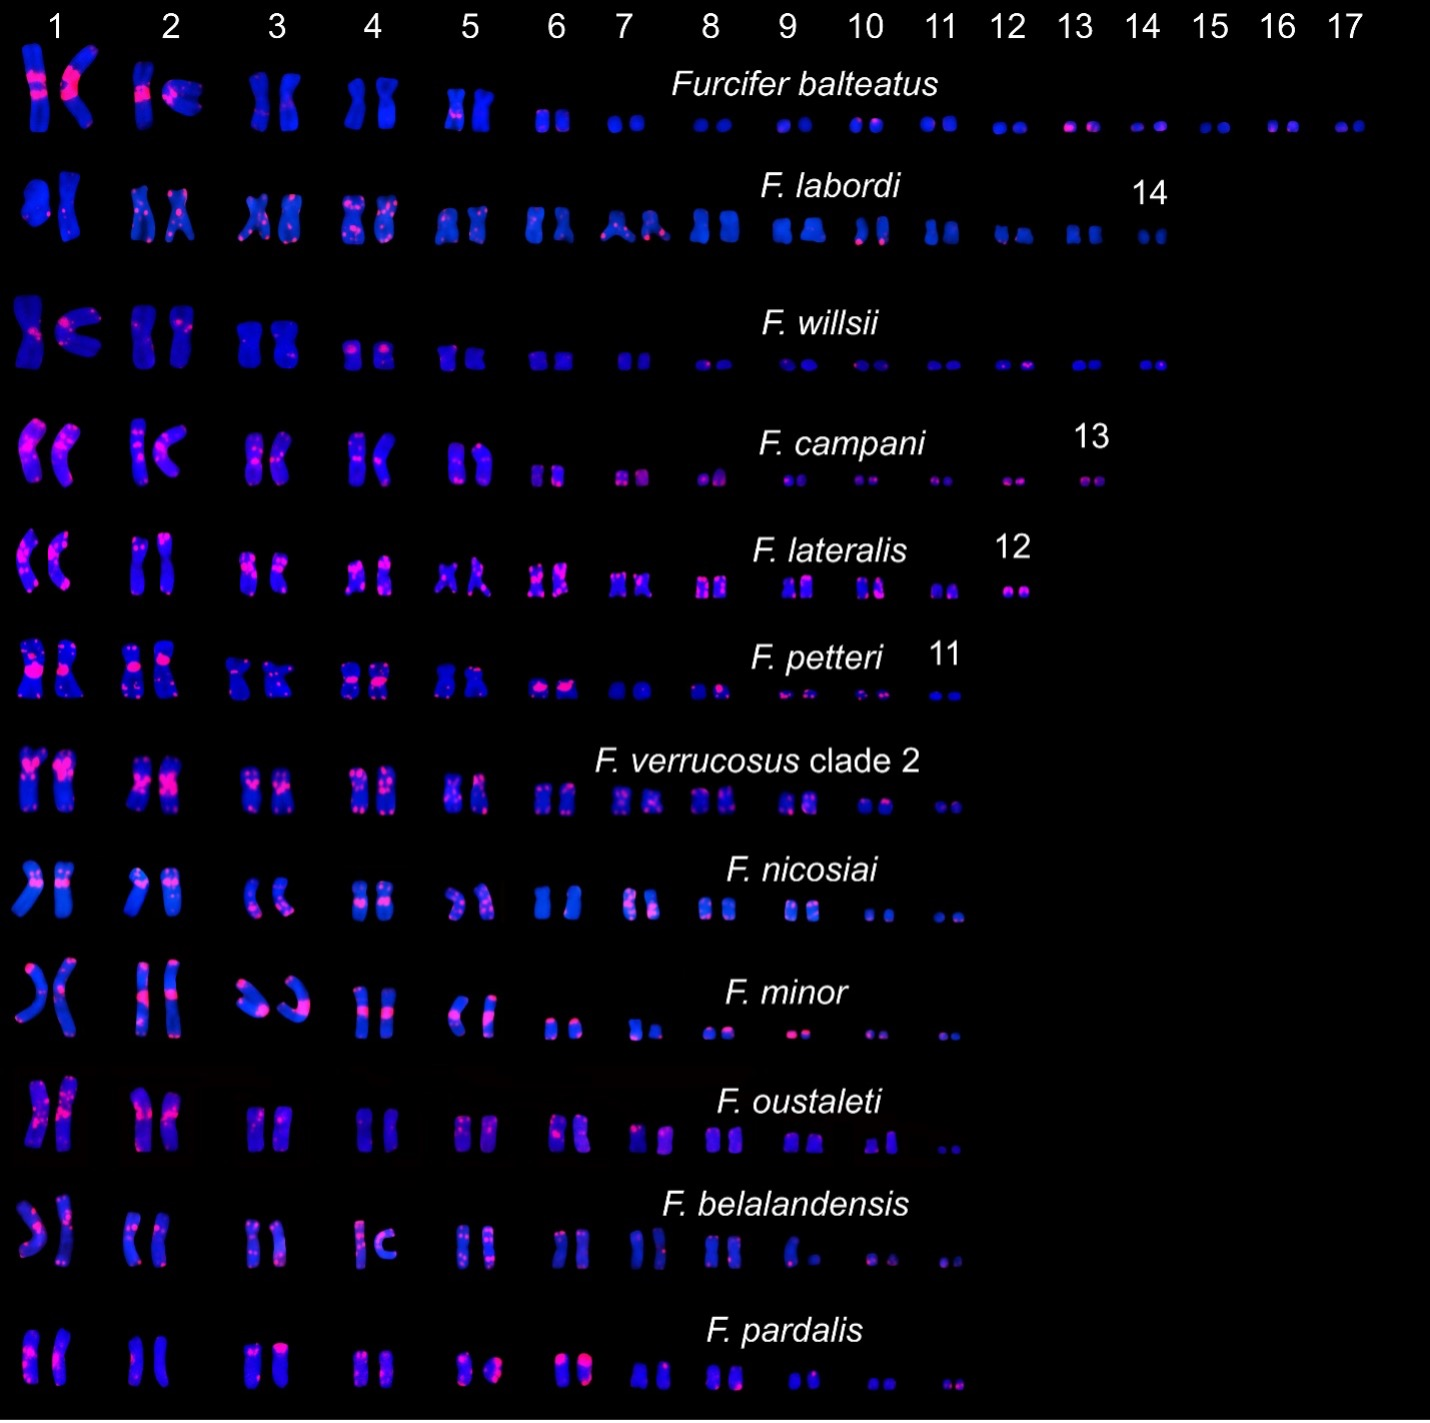
\includegraphics[width = \linewidth]{figures/marcello-s6.jpg}
  \caption{Karyotypes of \textit{Furcifer} stained with TELO-FISH.
}
  \label{fig-s6}
\end{figure}

%-------------------------------------------------------------------------------
% Refs
%----------------------------------------
\newpage
\section{Supplementary References}
 
\bibliography{chameleons}
\bibliographystyle{bibstyle}

\end{document}